\documentclass{article}
\usepackage[utf8]{inputenc}
\usepackage{amsfonts}
\usepackage{amsmath}
\usepackage{mathrsfs}
\usepackage{amsthm}
\usepackage[shortlabels]{enumitem}
\usepackage{graphicx}
\usepackage{xcolor}
\usepackage{mdframed}
\usepackage{float}
\usepackage[margin=0.75in]{geometry}
\usepackage{subfigure}
\definecolor{problem}{rgb}{0.8,0.8,0.8}
\newcommand{\comp}[2]{
\vspace{0.2in}\begin{mdframed}[
  backgroundcolor=problem,
  skipabove=\topsep,
  skipbelow=\topsep
  ]
  \emph{Computation {#1}:} {#2}
\end{mdframed}}
\newcommand{\exercise}[2]{
\vspace{0.2in}\begin{mdframed}[
  backgroundcolor=problem,
  skipabove=\topsep,
  skipbelow=\topsep
  ]
  \emph{Exercise {#1}:} {#2}
\end{mdframed}}
\newcommand{\R}{\mathbb{R}}
\newcommand{\N}{\mathbb{N}}
\newcommand{\Z}{\mathbb{Z}}
\newcommand{\Q}{\mathbb{Q}}
\newcommand{\C}{\mathbb{C}}
\newcommand{\ep}{\varepsilon}
\newcommand{\LIM}{\mathop{\textup{LIM}}}

\usepackage{fancyhdr}

\pagestyle{fancy}
\fancyhf{}
\rhead{Aidan Copinga, MATH6420}
\begin{document}
    % \exercise{1}{Solve the IVP/IBPs using the method of characteristics.}
    % \begin{enumerate}[(a)]
    %   \item Let $b\in \R^n,c\in \R$ find the general solution of,
    %   \[\begin{cases}
    %     u_t + b\cdot D_x u = cu &(x,t)\in \R^n\otimes (0,\infty) \\
    %     u(x,0)=g(x) &x\in\R^n
    %   \end{cases}\]
    %   \item[] \textit{Solution:} This has characteristic equations
    %   \begin{align*}
    %     \frac{\partial x}{\partial s} = b,\,\,
    %     \frac{\partial t}{\partial s} = 1,\,\,
    %     \frac{\partial u}{\partial s}=cu
    %   \end{align*}
    %   subject to the initial conditions
    %   \begin{align*}
    %     x(0) = \xi,\,\,
    %     t(0) = 0,\,\,
    %     u(0) = g(\xi)
    %   \end{align*}
    %   This has the following solutions
    %   \begin{align*}
    %     x(s,\xi) = bs + \xi,\,\, t(s,\xi) = s,\,\,u(s,\xi) = g(\xi)e^{cs}
    %   \end{align*}
    %   Now change of variables lends
    %   \[s = t,\,\,\xi = x - bt\]
    %   so we have that $u(x,t) = g(x-bt)e^{ct}$.
    %   \item Find the general solution of
    %   \[\begin{cases}
    %     u_t + xu_x = 0 &(x,t)\in \R\otimes (0,\infty) \\
    %     u(x,0)=g(x) &x\in\R.
    %   \end{cases}\] 
    %   \item[] \textit{Solution:} This has characteristic equations
    %   \begin{align*}
    %     \frac{\partial x}{\partial s} = x,\,\,
    %     \frac{\partial t}{\partial s} = 1,\,\,
    %     \frac{\partial u}{\partial s}=0
    %   \end{align*}
    %   subject to the initial conditions
    %   \begin{align*}
    %     x(0) = \xi,\,\,
    %     t(0) = 0,\,\,
    %     u(0) = g(\xi)
    %   \end{align*}
    %   This has the following solutions
    %   \begin{align*}
    %     x(s,\xi) = \xi e^s,\,\, t(s,\xi) = s,\,\,u(s,\xi) = g(\xi)
    %   \end{align*}
    %   Now change of variables lends
    %   \[s = t,\,\,\xi = xe^{-t}\]
    %   so we have that $u(x,t) = g(xe^{-t})$.
    %   \item Find the general solution of
    %   \[\begin{cases}
    %     u_t + bu_x = 0\,\,\mathrm{for}\,\,(x,t)\in (0,\infty)\otimes (0,\infty) \\
    %     u(x,0)=f(x)\,\,\mathrm{and}\,\,u(0,t)=g(t).
    %   \end{cases}\] 
    %   \item[] \textit{Solution:} This has characteristic equations
    %   \begin{align*}
    %     \frac{\partial x}{\partial s} = b,\,\,
    %     \frac{\partial t}{\partial s} = 1,\,\,
    %     \frac{\partial u}{\partial s}=0
    %   \end{align*}
    %   subject to the initial conditions
    %   \begin{align*}
    %     x(0) = \xi,\,\,
    %     t(0) = 0,\,\,
    %     u(0) = f(\xi)
    %   \end{align*}
    %   This has the following solutions
    %   \begin{align*}
    %     x(s,\xi) = b\xi,\,\, t(s,\xi) = s,\,\,u(s,\xi) = f(\xi)
    %   \end{align*}
    %   Now change of variables lends
    %   \[s = t,\,\,\xi = x - bt\]
    %   so we have that $u(x,t) = f(x - bt)$. However, this is only along the characteristic line $t = 0$, along the characteristic
    %   $x = 0$, we need to determine boundary behaviour. Take characteristic $x(t) = \xi + bt$, now choose $t^\star$ s.t. $x(t^\star) = 0$.
    %   We see that $\xi = - bt^\star$, so substituting this into $x(t)=\xi + bt$, we see that $t^\star = t - x(t)/b$. This means we have 
    %   $u(x,t) = g(t - x/b)$ along $t - x/b > 0$.\newline
    %   When $b<0$, characteristic lines $\xi = x - bt$ pass through both boundaries $t = 0$ and $x = 0$. Assuming such a solution exists, this would imply that 
    %   solutions $u(x,t) = f(x-bt)$ agree with $f(-bt) = g(t)$ or $u(x,t) = g(t-x/b)$ agree with $g(-x/b) = f(x)$. If this were not the case, then any
    %   solutions would not exist.
    %   \item Find the general solution of
    %   \[\begin{cases}
    %     u_t + \sqrt{x}u_x = 0\,\,\mathrm{for}\,\,(x,t)\in (0,\infty)\otimes (0,\infty) \\
    %     u(x,0)=f(x)\,\,\mathrm{and}\,\,u(0,t)=g(t).
    %   \end{cases}\] 
    %   \item[] \textit{Solution:} This has characteristic equations
    %   \begin{align*}
    %     \frac{\partial x}{\partial s} = x^{1/2},\,\,
    %     \frac{\partial t}{\partial s} = 1,\,\,
    %     \frac{\partial u}{\partial s}=0
    %   \end{align*}
    %   subject to the initial conditions
    %   \begin{align*}
    %     x(0) = \xi,\,\,
    %     t(0) = 0,\,\,
    %     u(0) = f(\xi)
    %   \end{align*}
    %   This has the following solutions with $x > 0$,
    %   \begin{align*}
    %     x(s,\xi) = \frac{1}{4}(s + 2\sqrt{\xi})^2,\,\, t(s,\xi) = s,\,\,u(s,\xi) = f(\xi)
    %   \end{align*}
    %   Now change of variables lends
    %   \[s = t,\,\,\xi = \left(\sqrt{x}-\frac{t}{2}\right)^2\]
    %   Here, we see that when $\xi = 0$, $x = \left(\frac{t}{2}\right)^2$, so when $x < \left(\frac{t}{2}\right)^2$, we have that
    %   $u(x,t) = f(\left(\sqrt{x}-\frac{t}{2}\right)^2)$. Then when $x > \left(\frac{t}{2}\right)^2$, we see that $x(t) = \left(\sqrt{\xi}+\frac{t}{2}\right)^2$, so for $t^\star$ s.t. $\left(\sqrt{\xi} + \frac{t^\star}{2}\right)^2 = 0$
    %   so we have that $-\sqrt{\xi} = \left(\frac{{t^\star}}{2}\right)$, meaning that $t^\star = -2\sqrt{x} + t$ so then we have the solution $u(x,t) = g(t-2\sqrt{x})$.
    % \end{enumerate}
    % \exercise{2}{Use the method of characteristics to solve the following equation
    % \[\begin{cases}
    %   u_t + x|x|u_x = 0 &(x,t)\in \R\otimes(0,\infty) \\
    %   u(x,0) = f(x) &x\in\R
    % \end{cases}\]
    % After finding the general solution, suppose additionally that $f(x)=0$ for $|x|\le r$. Show that there is minimal time $T(r)$ so that for any such $f$ the corresponding solution $u$ satisfies $u(\dot,t)\equiv 0$ for all $t\ge T$, calculate $T(r)$.}
    % \textit{Solution:} This has characteristic equations
    % \begin{align*}
    %   \frac{\partial x}{\partial s} = x|x|,\,\,
    %   \frac{\partial t}{\partial s} = 1,\,\,
    %   \frac{\partial u}{\partial s}=0
    % \end{align*}
    % subject to the initial conditions
    % \begin{align*}
    %   x(0) = \xi,\,\,
    %   t(0) = 0,\,\,
    %   u(0) = f(\xi)
    % \end{align*}
    % This has the following solutions
    % \begin{align*}
    %   x(s,\xi) = \pm\frac{\xi}{\xi s \pm 1},\,\, t(s,\xi) = s,\,\,u(s,\xi) = f(\xi)
    % \end{align*}
    % Now change of variables lends
    % \[s = t,\,\,\xi = \mp\frac{x}{1\mp tx}\]
    % so when $\xi \ge 0$, we have that $\xi = \frac{x}{1+tx}$ as $\xi \ge 0$ implies that $\dot{x} \ge 0$. Now when $\xi < 0$, we have that $\xi = -\frac{x}{1-tx}$. Now we have the solution
    % \[u(x,t) = \begin{cases}
    %   f(\frac{x}{1+tx}) &x\ge 0\\
    %   f(-\frac{x}{1-tx}) &x\le 0.
    % \end{cases}\]
    % Given that $f(x) = 0$ for $|x| \le r$, we see that as $t \to \frac{1}{\mathrm{sgn}{(\xi)}\xi}$, solutions blow up. Consider when 
    % $t > \frac{1}{\mathrm{sgn}{(\xi)}\xi}$. Now it's sufficient to show that there is a $t^\star$ such that $x(t^\star,\xi) = r$ along the characteristic.
    % \begin{align*}
    %   r &= \pm\frac{\xi}{\xi t^\star \pm 1}\\
    %   \mp r(\xi t^\star \pm 1) &= \xi\\
    %   \xi t^\star \pm 1 &= \mp\frac{\xi}{r} \\
    %   t^\star &= \mp \left(\frac{1}{r} +\frac{1}{\xi}\right)
    % \end{align*}
    % so we see that $t^\star = \left(\frac{1}{r} +\frac{1}{|\xi|}\right)$ is such $t^\star$ so now, to show there is a minimal $T(r)$, we see that $\lim_{|\xi|\to\infty} t^\star = \frac{1}{r}$, so it has a minimal time $1/r$ where $u(x,t) = 0$ for all $t \ge 1/r$. 
    % \exercise{3}{Let $U$ be a bounded domain of $\R^n$. We say $u\in C^2(U)$ is subharmonic if $-\Delta u \le 0$ in $U$.
    % \begin{enumerate}[(a)]
    %   \item Prove for subharmonic $v$ that\[ v(x) \le \frac{1}{|B(x,r)|}\int_{B(x,r)}v(y)dy\,\,\text{ for all $\overline{B(x,r)}\subset U$.}\]
    %   \item Prove that the weak maximum principle holds for subharmonic $v\in C^2(U)\cap C(\bar{U})$.
    %   \item Let $\phi: \R\to\R$ be smooth and convex. Assume $u$ is harmonic and $v=\phi(u)$. Prove that $v$ is subharmonic.
    %   \item Prove $v=|Du|^2$ is subharmonic whenever $u$ is harmonic.
    % \end{enumerate}
    % }
    % \textit{Solution:}
    % \begin{enumerate}[(a)]
    %   \item It's sufficient to show that $v(x) \le \frac{1}{|B(x,r)|}\int_{\partial B} v(y)dy$ as 
    %   \[\frac{1}{|B(x,r)|}\int_{B} v(y)dy = \frac{1}{|B(x,r)|}\int_0^r d\rho\int_{\partial B} v(y)dy = \frac{1}{|B(x,r)|}\int_{\partial B} v(y)dy.\] Let $\phi(r) = \frac{1}{|B(x,r)|}\int_{\partial B} v(y)dy$. Now we see that (using $\int$ for the mean value integral because I'm not sure how to do that in LaTeX.)
    %   \[\phi'(r) = \int_{\partial B(0,1)} Dv(x+rz)\cdot zdS(z)\] letting $y = x+rz$. Using green's theorem, we see that (using the fact that $\Delta v \ge 0$)
    %   \[ \phi'(r) = \int_{\partial B(0,1)} Dv(x+rz)\cdot \frac{y-z}{r}dS(y) = \frac{r}{n}\int_{B(x,r)}\Delta v(y)dy \ge 0.\]
    %   Because $\phi' \ge 0$, we see that it's increasing,
    %   \[ \phi(r) = \int_{\partial B(x,r)}v(y)dy\ge v(x).\]
    %   \item Let $v \in C^2(U)\cap C(\bar{U})$. FSoC, suppose 
    %   \[\max_{x\in\bar{U}} v(x) > \max_{x\in\partial\bar{U}}v(x).\]
    %   Now, there is a point $x_0\in U$ s.t. $v(x_0) > \max_{x\in\partial\bar{U}}{v(x)}$.\newline
    %   By part (a), for any $r > 0$ for $B(x_0,r)\subset U$, 
    %   \[\int_{B(x_0,r)} v(y) - v(x_0)dy \ge 0\]
    %   but $v(y)-v(x_0)$ is nonpositive so $v(y)=v(x_0)$ for all $y\in B(x_0,r)$. Consider $L = \{r > 0|B(x_0,r)\subset U\}$ and $s=\sup{L}$. 
    %   Since $B(x_0,s)=\cup_{r\in L}B(x_0,r)\subset U$, we have that for all $y\in B(x_0,s),v(y)=v(x_0)$.\newline
    %   It's now sufficient to show that $\overline{B(x_0,s)}\cap \partial U\ne \emptyset$.\newline
    %   \textit{Proof of Above:} Suppose $\overline{B(x_0,s)}\cap \partial U$ is empty. Since $\cap{B(x_0,s)}\subset \bar{U}$, then $\overline{B(x_0,s)}\cap (\R^n\setminus U)$ is also empty.
    %   Since the ball is compact (Heine-Borel) and $\R^n\setminus U$ is closed, then 
    %   \[0 < \inf\{|b-a|\,\,|b\in \overline{B(x_0,s)},\,\,\,a\in(\R^n\setminus U)\} = d.\]
    %   However, this means that $B(x_0,s+d/2)\subset U$. But this means $s + d/2\in L$ and $s + d/2 > s = \sup{L}$, which is a contradiction.
    % \item $\phi$ is smooth and convex and $u$ is harmonic. $v = \phi(u)$ so
    % \begin{align*}
    %   \Delta v&= \nabla \cdot (\nabla v) \\
    %   \nabla v &= \phi'(u)\nabla u \\
    %   \nabla\cdot (\nabla v) &= \nabla\cdot(\phi'(u)\nabla u) \\
    %   &= (\phi''(u)\nabla u)\cdot\nabla u + \phi'(u)\nabla\cdot(\nabla u) \\
    %   &= (\phi''(u)\nabla u)\cdot\nabla u = \phi''(u)|\nabla u|^2\ge 0
    % \end{align*}
    % because $\phi$ is convex, it has $\phi'' \ge 0$. This implies that $-\Delta v \le 0$, and thus $v$ is subharmonic.
    % \item Since $u$ is harmonic, $u_{x_i}$ for $i=1,\dots,n$ is harmonic as well. $(u_{x_i})^2$ is subharmonic by (c). Now 
    %  \[|Du|^2 = \sum_{i=1}^n (u_{x_i})^2\]
    %  which is subharmonic as it's the sum of subharmonic functions.
    % \end{enumerate}

    % \exercise{4}{If $u$ is weakly harmonic, then $u$ is $C^2$ and harmonic.}
    % \textit{Solution:} Because $u$ is weakly harmonic, for test functions $\phi\in C^\infty_c$,
    % \[\int_{U}u\Delta\phi dx = 0.\]
    % Define a mollifier $\eta$ s.t. 
    % \[\eta(x) :=\begin{cases}
    % C\exp{\left(\frac{1}{|x|^2-1}\right)} &\mathit{if}\,\,|x|<1 \\
    % 0 &\mathit{if}\,\, |x|\ge 1
    % \end{cases}\]
    % Where $C$ is chosen such that $\int_{\R^n}\eta dx = 1$. Then, we can define $u_\epsilon = \eta_\epsilon \star u$. Now, for $\epsilon > 0$ set
    % \[\eta_\epsilon(x) := \frac{1}{\epsilon^n}\eta\left(\frac{x}{\epsilon}\right)\]
    % Now define the set $U_\epsilon := \{x\in U\,\,:\,\,d(x,\partial U) > \epsilon\}$ where $d$ is the distance metric.
    % Because $\eta_\epsilon$ is supported on $B(0,\epsilon)$, we see that $\eta_\epsilon(x-y)$ is compactly supported in $U$ for any $x\in U_\epsilon$.\newline
    % Fix $x \in U_\epsilon$, and because $u$ is continuous and $\eta_{\epsilon}(x-y)$ being continuously differentiable,
    % \begin{align*}
    %   \Delta u_\epsilon &= \Delta_x (\eta_\epsilon \star u)\\
    %   &= \Delta_x \int_{\R^n}\eta_\epsilon(x-y)u(y)dy \\
    %   &= \Delta_x \int_{U} \eta_{\epsilon}(x-y)u(y)dy \\
    %   &= \int_U\Delta_x \left[\eta_\epsilon(x-y)\right]u(y)dy \\
    %   &= \int_U\Delta y \left[\eta_\epsilon(x-y)\right]u(y)dy \\
    %   &= \int_U\Delta \phi udy \\
    %   &= 0
    % \end{align*}
    % where $\phi = \eta_\epsilon(x-y)$. We see that $\Delta u_\epsilon$ is harmonic.
    % Now, choose $\epsilon_2 > 0$ and set $u_{\epsilon\epsilon_2} := \eta_{\epsilon_2}\star u_\epsilon$. We see that $\eta_{\epsilon_2}(x-y)$ is compactly supported on $U_{\epsilon}$ for $x\in U_{\epsilon + \epsilon_2}$.
    % Computing in polar coordinates gives
    % \begin{align*}
    %   u_{\epsilon\epsilon_2} &= \int_{U_\epsilon}\eta_{\epsilon_2}(x-y)u_\epsilon(y)dy \\
    %   &= \frac{1}{\epsilon_2^n}\int_{B(x,\epsilon_2)}\eta\left(\frac{|x-y|}{\epsilon_2}\right)u_\epsilon(y)dy \\
    %   &= \frac{1}{\epsilon_2^n}\int_0^{\epsilon_2}\eta\left(\frac{r}{\epsilon_2}\right)\int_{\partial B(x,r)}u_\epsilon(y)dS(y)dr \\
    %   &= u_\epsilon(x)\int_{B(x,\epsilon)}\eta\left(\frac{x-y}{\epsilon_2}\right)dy \\
    %   &= u_\epsilon(x)\int_{B(0,\epsilon)}\eta\left(y\right)dy \\
    %   &= u_\epsilon(x)
    % \end{align*}
    % Because convolution is associative, for $x\in U_{\epsilon+\epsilon_2}$, we have that $u_{\epsilon_2\epsilon} = u_{\epsilon\epsilon_2} = u_\epsilon \to u(x)$ uniformly. Furthermore,
    % \[u(x) = u_{\epsilon_2}(x)\] so we can conclude that for each $\epsilon,\epsilon_2$, $u = u_{\epsilon_2} \in C^\infty(U_{\epsilon + \epsilon_2})$ and harmonic.
    % \exercise{5}{Let $U$ be a bounded domain of $\R^n$ and $u\in C^2(U)\cap C(\overline{U})$ which is harmonic in $U$. Suppose that $u(x_0)=\min_{\overline{U}}u=0$ at some 
    % $x_0\in \partial U$. Suppose that there exists $x_1$ so that $B(x_1,r)\in U$ an $\partial(x_1,r)\cap\partial U = \{x_0\}$. Prove that if $u$ is not constant, then 
    % \[ \frac{\partial u}{\partial \upsilon}(x_0) < 0\]
    % where $\upsilon$ is the outward unit normal to $B(x_1,r)$ at $x_0$.}
    % \textit{Solution:} 
    % The solution $v = -u$ is still harmonic in the same domain $U$, so by the Strong maximum principle because $u =-v$ is not constant, $v(x_0) = 0$ is a maximum of $v$ and hence $v < 0 \in U$. 
    % Furthermore, $u > 0$ in $U$.\newline
    % Because $u$ is harmonic and positive, we have that by poisson's formula, for $R > r$, 
    % \[u(x) = \frac{1}{\alpha(n)}\int_{B(x_1,r)}\frac{R^2-r^2}{R|x_1-y|^n}u(y)dy\] 
    % The kernel in the integrand has 
    % \[ \frac{R-r}{R(R+r)^{n-1}}\le \frac{R^2-r^2}{R|x-y|^n}.\]
    % Harnack's Inequality follows with
    % \[ \frac{R-r}{\alpha(n)R(R+r)^{n-1}}\int_{B(x_1,r)}u(y)dy\le \frac{1}{\alpha(n)}\int_{B(x_1,r)}\frac{R^2-r^2}{R|x_1-y|^n}u(y)dy\]
    % It then follows from the mean value property that
    % \[ \frac{R-r}{R(1+(r/R))^{n-1}}u(x_1)\le u(x)\]
    % for every point $|x-x_1|<r\le R$. This result is satisfied by Poisson's formula and the mean value property (as the general statement is proved in Evans.)\newline
    % The limit 
    % \[\limsup_{h\to 0} \frac{u(x_0)-u(x_0-h\upsilon)}{h}\]
    % by change of variables can be changed to
    % \[\limsup_{r\to R} \frac{u(x_0)-u(x_0\left(\frac{r}{R}\right))}{R-r}\]
    % (Instead of looking at $u$ at the point $x_0-h\upsilon$, the latter looks at the point $rx_0/R$ as $r\to R$, which is looking in the opposite direction.)
    % We see that
    % \[\frac{-u(x_0\left(\frac{r}{R}\right))}{R-r} \le  -\frac{1}{R-r}\frac{R-r}{(1+(r/R))^{n-1}}u(x_1) = -\frac{1}{(1 + (r/R))^{n-1}}u(x_1) < -\frac{1}{2^{n-1}}u(x_1) < 0.\]
    % So clearly its $\limsup$ is negative, and hence, has a negative directional derivative at $x_0$.
    % \exercise{6}{Let $U$ be a bounded domain of $\R^n$ with $C^2$ boundary, in particular it has an interior tangent ball at every boundary point. Use the result of the previous problem to show that any two solutions of the Neumann problem
    % \[\begin{cases}
    %   -\Delta u = f &\text{in}\quad U \\
    %   \frac{\partial u}{\partial \upsilon} = h &\text{on}\quad \partial U
    % \end{cases}\]
    % differ by a constant.}
    % Consider $u_1,u_2$ solutions to the above. Now consider $\omega = u_2 - u_1$. We see that
    % \[\begin{cases}
    %   -\Delta \omega = 0 &\text{in}\quad U \\
    %   \frac{\partial \omega}{\partial \upsilon} = 0 &\text{on}\quad \partial U
    % \end{cases}\]
    % So $\omega$ is harmonic, so using Green's we see that
    % \[\int_U \omega\Delta\omega dx = \int_{\partial U}\omega\frac{\partial \omega}{\partial \upsilon} dS(\upsilon) - \int_U |\nabla \omega|^2dx.\]
    % Since $\frac{\partial \omega}{\partial \upsilon} = \Delta \omega = 0$, 
    % \[\int_U |\nabla \omega|^2dx = 0 \implies \omega \text{ constant.}\]
    % Hence $u_2 = u_1 + \text{ constant}$.
    % \exercise{7}{Let $U$ be a bounded domain of $\R^n$ and $b:\overline{U}\to \R^n$ be continuous. Prove there is at most one solution $u\in C^2(U)\cap C(\overline{U})$ of the Dirichlet problem,
    % \[\begin{cases}
    %   -\Delta u + b(x) \cdot \nabla u = f(x) &\text{in } U \\
    %   u=g(x) &\text{on } \partial U.
    % \end{cases}\]}
    % \textit{Solution:} 
    % Assume $-\Delta u + b(x)\cdot\nabla u < 0$, and that $x\in \partial U$ is a maximum of $u(x)$. This means,
    % \[\Delta u = \sum \frac{\partial_{ii}^2u}{\partial x_{ii}^2} \le 0\]
    % where $x_{ij}$ is an entry of the Hessian matrix of second partial derivatives, and such $\Delta u \le 0$. Furthermore, because 
    % $u(x)$ is a maximum, it has that $D_{x_i} u(x) = 0$ for each $x_i$ (and hence $\nabla u(x) = 0$.) This means that
    % \[-\Delta u + b(x)\cdot \nabla u(x) = -\Delta u \ge 0\]
    % but by assumption, this is a contradiction.\newline
    % Now Assume $-\Delta u + b(x)\cdot\nabla u \le 0$, and that $x\in \partial U$ is a maximum of $u(x)$.
    % Introduce a perturbation term $v_\delta$ such that
    % \[v_\delta(x) = u(x) + \delta v(x).\]
    % Let $v(x_l): \overline{U}\to\R^n$ such that $v(x_l)=0$ for every $1 < l \le n$.
    % Now we have that
    % \begin{align*}
    %   -\Delta v_\delta + b(x)\cdot \nabla v_\delta(x) &= -\Delta u + b(x)\cdot \nabla u - \Delta \delta v + b(x)\cdot \nabla \delta v \\
    %   &<-\delta\Delta v + \delta b(x)\cdot\nabla v \\
    %   &= -\delta \frac{d^2 v}{dx_1^2} + \delta b(x_1)\frac{dv}{dx_1} < 0\star
    % \end{align*}
    % To show $\star$: because $b:\overline{U}\to\R^n$, let $B = \sup_{\overline{U}} |b(x_1)|$. Then, let $r < 0$ so that $-\frac{d^2 v}{dx_1^2} + B\frac{dv}{dx_1} = r$. We see that 
    % \[v(x_1) = c_1\frac{e^{Bx}}{B} + \frac{rx}{B} + c_2\]
    % WLOG, let $c_1=1, c_2=0$. Now we have that We see that $v_\delta = u + \delta v(x) \to u$ as $\delta \to 0$ uniformly on $U$, so the maximum is achieved on $U$ with 
    % \[u\le v_\delta \le u + \delta \max_{\overline{U}}\left(\frac{e^{Bx}}{B} + \frac{rx}{B}\right).\]
    % Let $w = u_1-u_2$ where $u_1,u_2$ are solutions of the above. We have that
    % \[-\Delta w + b(x)\cdot \nabla w = 0,\quad w = 0 \text{ on $\partial U$}\]
    % However, by the weak maximum principle proved just above, $w$ is 0 on the boundary so it must be a maximum, and hence $0$.
    % \exercise{10}{If $u$ is harmonic and 
    % \[\lim_{R\to\infty}\frac{1}{R^2}\sup_{B(0,R)} |u(x)| = 0,\]
    % show that $u$ is linear.}
    % By Theorem 2.2.7, estimate $|D^2u|$ by 
    % \[|D^2u|\le \frac{4(2^{n+1}n)^2}{R^2\alpha(n)R^n}\|u\|_{L^1}\]
    % Now, we can manipulate this given that $B(0,R)$ is bounded for each $R$.
    % \begin{align*}
    %   |D^2u|&\le \frac{4(2^{n+1}n)^2}{R^2\alpha(n)R^n}\|u\|_{L^1} \le \frac{4(2^{n+1}n)^2}{R^2}\|u\|_{L^\infty} = \frac{4(2^{n+1}n)^2}{R^2}\sup_{B(0,R)} |u(x)|
    % \end{align*}
    % We now see that we have the second derivative of $u$ bounded by 
    % \[\frac{C}{R^2}\sup_{B(0,R)} |u(x)|\]
    % so this clearly tends towards 0 by assumption. Hence, $u(x)$ is linear.
    % \exercise{12}{Consider the problem of minimizing the Dirichlet energy
    % \[I[v] = \int_U|Dv|^2dx\]
    % over the admissable class 
    % \[\mathcal{A} = \left\{v\in C^2(\overline{U}):v\vert_{\partial U} = 0\,\,\text{and}\,\,\int_U|v|^2dx=1.\right\}\]
    % Show that if $u$ satisfies 
    % \[I[u]=\min I[v]\]
    % then $u$ solves the Dirichlet eigenvalue problem with eigenvalue $\lambda_0=\min I[v]$. Show that if $\lambda_1$ is another eigenvalue of the Dirichlet Laplacian on $U$, then $\lambda_1\ge \lambda_0$.}
    % \begin{proof}[Solution]
    % Because $u$ minimizes $I[v]$, let $v\in C^\infty_c(U)$
    % \[i[\tau] := I\left[\frac{u + \tau v}{\|u+\tau v\|_{L^2}}\right].\]
    % We see that each $\frac{u + \tau v}{\int_{U}|u+\tau v|^2}\in\mathcal{A}$ for each $\tau$, the scalar function $i$ has a minimum at 0, and thus
    % \[i_\tau(0)=0.\]
    % Then $i(\tau)$ has 
    % \[ i(\tau) = \frac{1}{\|u+\tau v\|_{L^2}^2}\int_U|Du + \tau Dv|^2dx = \frac{1}{\int_U|u|^2 + 2\tau|uv|+|v|^2dx}\int_U |Du|^2 + 2\tau Du\cdot Dv + \tau^2|Dv|^2dx\]
    % So we see that 
    % \[0 = i'(0) = \frac{1}{\|u\|_{L^2}^2}\int_U Du\cdot Dv dx + \frac{-\int_Uuvdx}{\|u\|_{L^2}^4}\int_U|Du|^2dx= \int_U (-\Delta u) v dx - \frac{\int_Uuvdx}{\|u\|_{L^2}^2}\int_U|Du|^2dx\]
    % Now we see that, if we allow $u\in\mathcal{A}$,
    %   \[0=\int_U (-\Delta u)vdx - \int_Uuvdx \int_U|Du|^2dx =\int_U (-\Delta u)vdx - \int_U(I[u]u)vdx.\]
    %   So $-\Delta u = \lambda_0u$ with $\lambda_0 = I[u]$.\newline
    %   Now let $\lambda_1$ is another eigenvalue of the Dirichlet problem, with $w\in C^2(\overline{U})$ so
    %   \begin{equation}\label{eq:Dirich}
    %     \begin{cases}
    %     -\Delta w = \lambda_1 w &x\in U\\
    %     w = 0 &x\in\partial U
    %   \end{cases}.\end{equation}
    %   Then a normalized $w_2 = \frac{1}{\|w\|_{L^2}}w$ is a solution to \eqref{eq:Dirich} as
    %   \begin{align*}
    %     \Delta \left(\frac{1}{\|w\|_{L^2}}w\right) = \frac{1}{\|w\|_{L^2}}\Delta w
    %   \end{align*}
    %   by linearity of the Laplacian. Furthermore, $w_2\in \mathcal{A}$, so if $w_2 = u$, we see that $\lambda_0 = \lambda_1$ by the argument above.
    %   However, when $w_2\ne u$, we see that if $\lambda_1 < \lambda_0$, then $\int_U |Dw_2|^2dx < \int_U |Du|^2dx$, which is a contradiction, so $\lambda_0 \le \lambda_1$.
    % \end{proof}
    % \exercise{13}{Consider the problem of minimizing the Dirichlet energy
    % \[I[v] = \int_U\frac{1}{2}|Dv|^2-fvdx\]
    % over the admissable class 
    % \[\mathcal{A} = C^2(\overline{U})\]
    % Show that if $u$ satisfies 
    % \[I[u]=\min I[v]\]
    % then $u$ solves the Neumann problem.}
    % \begin{proof}[Solution]
    % Because $u$ minimizes $I[v]$, let $v\in C^\infty_c(U)$ so $v$ vanishes on $\partial U$,
    % \[i[\tau] := I\left[u + \tau v\right].\]
    % We see that each $u + \tau v\in\mathcal{A}$ for each $\tau$, the scalar function $i$ has a minimum at 0, and thus
    % \[i_\tau(0)=0.\]
    % Then $i(\tau)$ has 
    % \[ i(\tau) = \int_U\frac{1}{2}|Du + \tau Dv|^2 - (u+\tau v)fdx = \int_U \frac{1}{2}|Du|^2 + \tau Du\cdot Dv + \frac{\tau^2}{2}|Dv|^2 - (u+\tau v)fdx\]
    % So we see that 
    % \[0 = i'(0) = \int_U Du\cdot Dv - vf dx = \int_U (-\Delta u-f)vdx\]
    % which is $0$ whenever $\Delta u = f$. Now, in order to show that the boundary conditions are satisfied, allow $w\in C^\infty_c(\overline{U}).$
    % We know that in $U$, $u + \tau w$ minimizes $I$, and is a solution, so $-\Delta u = f$. Furthermore, taking the derivative w.r.t $\tau$ like before, we see that
    % \[0= \int_{U} Du\cdot Dw - wfdx = \int_{\partial U} w\frac{du}{d\nu} dS - \int_U (-\Delta u - f)wdx = \int_{\partial U} w\frac{du}{d\nu} dS.\]
    % This implies that $\frac{du}{d\nu}$ needs to vanish on $\partial U$, so the Neumann boundary condition is satisfied.
    % \end{proof}
    % \exercise{14}{Let $u$ be the solution of the Dirichlet problem on $U = \R_+^n$ given by the Poisson formula for the half-space. $g$ is bounded and $g(x) = |x|$ for $x\in\partial\R^n_+$. Show $Du$ is not bounded near $x=0$.}
    % \[u(x) = \frac{2x_n}{n\alpha(n)}\int_{\partial \R^n_+}\frac{g(y)}{|x-y|^n}dS(y).\] Let $x = \lambda e_n = [0,0,\dots,\lambda]$. Now we see that
    % Following the hint, note that $u(0)=g(0)= 0$, so we estimate the derivative $Du$ with $x$, 
    % \begin{align*}
    %   \frac{(u(x) - u(0))}{\lambda} = \frac{2e_n}{n\alpha(n)}\int_{\partial \R_+^n}\frac{|y|}{|\lambda + |y||^n}dS(y).
    % \end{align*}
    % Now consider the integral over $\Omega = \partial\R_+^n \cap \{|y|\le 1\}$ with
    % \begin{align*}
    %   \frac{(u(x) - u(0))}{\lambda} &=\frac{2e_n}{n\alpha(n)}\int_\Omega \frac{|y|}{|\lambda + |y||^n}dS(y) \\
    %   &= (n-1)\alpha(n-1)\int_0^1\frac{r^{n-1}}{|\lambda - r|^n}dr \\
    %   &= (n-1)\alpha(n-1)\int_0^1\frac{1}{r((\lambda/r)^2 - 1)^{n/2}}dr
    % \end{align*}
    % However, this integral diverges, hence $Du$ cannot be bounded as $Du\cdot x$ is unbounded as $\lambda\to 0$.
    % \exercise{16}{The Kelvin transform $\mathcal{K} u = \bar{u}$ of a function $u:\R^n\to \R$ is 
    % \[\bar{u}: u(x/|x|^2)|x|^{2-n}\]
    % with $\bar{x}=x/|x|^2$. Show that if $u$ is harmonic, then so is $\bar{u}$.}
    % First, compute $D_x\bar{x}$
    % \begin{align*}
    %   D_x\bar{x} = \frac{I|x|^2 - 2xx^T}{|x|^4}
    % \end{align*}
    % Now compute $D_x\bar{x}(D_x\bar{x})^T$
    % \begin{align*}
    %   D_x\bar{x}(D_x\bar{x})^T &= \frac{1}{|x|^8}(I|x|^2-2xx^T)(I|x|^2-2xx^T)^T \\
    %   &=\frac{1}{|x|^8}(I|x|^2-2xx^T)(I|x|^2-2xx^T) \\
    %   &= \frac{1}{|x|^8}(I|x|^4-4|x|^2xx^T+4|x|^2xx^T) = I/|x|^4 = |\bar{x}|^4I
    % \end{align*}
    % as $\left|\frac{x}{|x|}\right| = \left|\frac{1}{|x|}\right|$.\newline
    % Now, we compute as $\Delta \bar{x} = n(2-n)\frac{x}{|x|^4}$. Furthermore, we can compute $\Delta u(\bar{x})$ with
    % \[\Delta (u(\bar{x})) = \sum_{i=1}^n \partial_{x_i} \bar{x}^T D^2u(\bar{x})\partial_{x_i}\bar{x} + Du(\bar{x})^T\Delta \bar{x} = \text{Tr}((D\bar{x})^TD^2uD\bar{x}) + Du\cdot \Delta \bar{x}.\]
    % We see that $\text{Tr}((D\bar{x})^TD^2uD\bar{x}) = |\bar{x}|^4\Delta u$ from the hint above. Now, we compute $\Delta \bar{u}$ with chain rule,
    % \[\Delta \bar{u} = |\bar{x}|^{n-2}|\bar{x}|^4(\Delta u) + u(\bar{x})\Delta(|\bar{x}|^{n-2}) + 2DuD\bar{x}(D|\bar{x}|^{n-2})^T + |\bar{x}|^{n-2}Du\cdot\Delta \bar{x}.\]
    % The first two terms are equivalently $0$ because $\Delta |\bar{x}|^{2-n} = \sum_{j=1}^n (n-2)\left(1 - \frac{nx_j^2}{|x|^2}\right)$ and $u$ is harmonic.\newline
    % Now we see that 
    % \[2DuD\bar{x}(D|\bar{x}|^{n-2})^T = 2Du\left(|x|^{-2}\left(I - 2 \frac{xx^T}{|x|^2}\right)\right)(2-n)|x|^{-n}x^T = 2(n-2)|x|^{-2-n}Du\cdot x^T = -|\bar{x}|^{n-2}Du\cdot\Delta \bar{x}.\]
    % This term allows $\Delta \bar{u} = 0$ so the Kelvin transform of $u$ is also harmonic.
      % \exercise{17}{Let $U$ be a bounded domain in $\R^n$ and $\alpha \in (0,1)$. Suppose that $u\in C^2(U)\cap C(\overline{U})$ solves 
      % \[\begin{cases}
      %   -\Delta u = |u|^\alpha &\text{in } U\\
      %   u(x) = 0 &\text{on } \partial U.
      % \end{cases}\]
      % Show that 
      % \[ \sup_U|u|\le C\]
      % where $C$ depends only on $n,\alpha$, and $\text{diam}(U)$.}
      % \begin{proof}[Solution]
      %   By Evans 2.6, using $x_0$ such that $U\subseteq B(x_0,\text{diam}(U))$,
      %   \[\max_{\bar{U}} |u| \le \frac{\max_{\overline{U}}|x-x_0|^2}{2n}\max_{\overline{U}}|u|^\alpha\]
      %   It follows that
      %   \[\max_{\bar{U}} |u| \le \frac{\max_{\overline{U}}|x-x_0|^2}{2n}\left(\max_{\overline{U}}|u|\right)^\alpha\]
      %   Furthermore, the ball $B(x_0, \text{diam}(U))$ contains $U$ and so 
      %   \[\max_{\bar{U}} |u| \le \frac{\text{diam}(U)^2}{2n}\left(\max_{\overline{U}}|u|\right)^\alpha\]
      %   Now, because $\max_{\bar{U}} |u| \ge 0$ and $0< \alpha < 1$, we can rearrange this to see that 
      %   \[ \max_{\bar{U}} |u| \le \left(\frac{\text{diam}(U)^2}{2n}\right)^{1/(1-a)}\]
      % \end{proof}
      % \exercise{18}{Consider the stationary Schrodinger operators.}
      % \begin{proof}[Solution]
      %   \begin{enumerate}
      %     \item We can let $V(x) = -\pi$ so then in $\R^1$, it solves the ODE 
      %     \[u'' = -\pi u\]
      %     which has solution $\sin(\pi x)$, so let this be on the interval $(0,1)\subset \R$. This violates maximum principle as $u(x)$ larger than 0 on its domain.
      %     \item By problem 2.6 in Evans, we see that 
      %     \[\max_{\overline{U}}|u| \le \frac{\text{diam}(U)^2}{2n}\max_{\overline{U}}(|V(x)u|) \le \frac{M\text{diam}(U)^2}{2n}\max_{\overline{U}}(|u|)\]
      %     Now, let $\delta = \sqrt{\frac{n}{M}}$, and we see that whenever $\text{diam}(U) \le \delta$
      %     \[ \max_{\overline{U}} |u| \le \frac{1}{2}\max_{\overline{U}}|u|\]
      %     which implies that $u = 0$
      %     \item Again, using problem 2.6 in Evans, this time fixing $x_2,\dots x_n$ and taking the maximum over $x_1,$
      %     \[\max_{x_1\in\overline{U}}|u| \le \frac{\text{diam}(U)^2}{2n}\max_{\overline{U}}(|V(x)u|) \le \frac{M\text{diam}(U)^2}{2n}\max_{x_1\in\overline{U}}(|u|)\]
      %     We see that because $x_2,\dots,x_n$ are fixed, $U\subseteq \{0 < x_1 < \text{diam}(U)\}$. Now, letting $\{0 < x_1 < \delta\}$ for $\delta = \sqrt{\frac{n}{M}}$, we see that 
      %     \[\max_{x_1\in\overline{U}}|u| \le \frac{1}{2} \max_{x_1\in\overline{U}}|u|\]
      %     Hence, $u(x)=0$ for any $x_1$, but this choice of $x_2,\dots x_n$ was arbitrary so $u = 0$ for all $x\in U$ such that $U \subset \{0 < x_1 < \delta\}$.
      %   \end{enumerate}
      % \end{proof}
      % \exercise{19}{Show that $u(x) = 0$ on the provided PDE.}
      % \begin{proof}[Solution]
      %   Let $u$ be a solution. Then, let $x_0\in U$ and $B(x_0,r)$ be the open ball of radius $r$. Now, consider the set 
      %   \[\overline{B(x_0,r)\cap U}\]
      %   By the maximum principle, there is a maximum on $\partial\overline{B(x_0,r)\cap U}$. Similarly, for $u$, there is a minimum on this set (maximum principle on $-u$). Now, 
      %   noticing that $r = |x-x_0|$, for $\epsilon > 0$, there is $r$ large enough such that $u(x) \le \epsilon$ on $\partial \overline{B(x_0,r)\cap U}$. 
      %   Moreover, on this set, $|u| \le \epsilon$, so as $r\to\infty$, $|u|(x) = 0$ which implies that $u(x)=0$.
         

      % \end{proof}
      % \exercise{20}{Show the comparison principle for 
      % \[-\Delta w + |Dw|^2 = 0\]}
      % \begin{proof}[Solution]
      %   Let $u$ be a strict subsolution so $-\Delta u + |Du|^2 < 0$ with $u < v$ on $\partial U$. Then, let $x_0$ be the maximal point of $u-v$ in $U$. 
      %   \[\max{(u-v)} \implies  \partial^2_{x}(u-v)(x_0) < 0, |D(u-v)|(x_0) = 0.\]
      %   However, this would means that $\Delta (u-v) < 0$, which is a contradiction as $-\Delta u < 0$ and $\Delta v = 0$. Furthermore, $u \le v$ in the boundary so $v - u$ is nonnegative in $U$.\newline
      %   Now let $-\Delta u + |Du|^2 = 0$ with perturbation $t_\epsilon(x) = \epsilon e^{-cx_1}$. We have that for $u + t_\epsilon$ 
      %   \begin{align*}
      %     -\Delta (u + t_\epsilon) + |Du + Dt_\epsilon|^2 &= -\Delta u + |Du|^2 -\Delta t_\epsilon + 2Du\cdot Dt_\epsilon + |Dt_\epsilon|^2 \\
      %     &= -\Delta t_\epsilon + 2Du\cdot Dt_\epsilon + |Dt_\epsilon|^2 \\
      %     &= -c^2\epsilon e^{-cx_1} -2c\epsilon u_{x_1}e^{-cx_1}+ c^2\epsilon^2e^{-2cx_1} \\
      %     &= -c^2\epsilon e^{-cx_1} -2c\epsilon u_{x_1}e^{-cx_1} + O(\epsilon^2)
      %   \end{align*}
      %   It's now sufficient to show that $-c^2\epsilon e^{-x_1} -2c\epsilon u_{x_1}e^{-x_1} < 0$ in order for $u$ to be approximated by strict subsolutions as $\epsilon$ can be made small enough such that the $c^2\epsilon^2e^{-2cx_1}$ term is smaller than the sum. 
      %   To do this, we just let $c = \frac{1}{\max\{u_{x_1}\}}$, so now we can make 
      %   \[-c^2\epsilon e^{-cx_1} -2c\epsilon u_{x_1}e^{-cx_1} + O(\epsilon^2) < 0\]
      %   for small enough $\epsilon > 0$. So we see that
      %   \[ -\Delta (u+t_\epsilon) + |D(u+t_\epsilon)|^2 < 0.\]
      %   Then by the proof for strict subsolutions, $u+t_\epsilon$ has that $u+t_\epsilon \le v$ in $U$, and letting $\epsilon\to 0$, we see that $u\le v$ in $U$.
      % \end{proof}
      % \exercise{21}{Show that $u(x) = 0$ for the provided Dirichlet problem.}
      % \begin{proof}[Solution]
      %   We know by the maximum principle that $u$ must be non-positive as it is $-1$ on the boundary $x=\{0\}$ and $0$ on the boundary $\partial B$. Let $\Phi(x)$ be the fundamental solution, then we define the function 
      %   \[v_j(x) = \max\left\{\frac{1}{j}\left(\Phi(1)-\Phi(x)\right), -1\right\}.\]
      %   $v$ is a subsolution because $-\Delta v \le 0$ and $v_j(0) = -1$ and $v_j = 0$ on $\partial B$. We see that if we let $j\to\infty$, then $v_j\to 0$ pointwise.\newline
      %   This sequence is non-decreasing, so the supremum of these subsolutions would $u(x)=0$.
      % \end{proof}
      % \exercise{25}{Show that 
      % \[\int \Phi(y,t)|y|^pdy \le Ct^{p/2}.\]}
      % \begin{proof}[Solution:]
      %   Substituting $z = \frac{y}{2\sqrt{t}}$ we have that
      %   \begin{align*}
      %     \int_{\R^n}\frac{1}{(2\pi t)^{n/2}}e^{-|y|^2/4t}|y|^pdy &= \int_{\R^n}\frac{1}{\pi^{n/2}}e^{-z^2}|2\sqrt{t}z|^pdz \\
      %     &= \left[\frac{2^p}{\pi^{n/2}}\int_{\R^n}e^{-|z|^2}|z|^pdz\right] t^{p/2}
      %   \end{align*}
      %   Because $|z|^p < O(e^{|z|^2}),$ the term in parantheses is finite, and always constant.
      % \end{proof}
      % \exercise{26}{Let $g:\R^n\to \R$ be boudned and $\alpha-$Holder continuous for some $\alpha\in (0,1]$. Show that for solutions of the heat equation $u(x,t)$ with initial data $g$,
      % \begin{equation}\sup_{x,t}|\partial_t u| + \sup_{x,t}\left\{\sum_{i,j}|\partial^2_{x_ix_j}u|\right\}\le C\sup_{x\ne y}\frac{|g(x)-g(y)|}{|x-y|^\alpha} t^{(\alpha/2) - 1}.\end{equation}}
      % \begin{proof}[Solution:]
      %   % By commutativity, we have that 
      %   % \[u(x,t) = \int_{\R^n} \Phi(y,t)g(x-y)dy\]
      %   % so for $x\ne x_0$, using the fact that $\Phi > 0$,
      %   % \[|u(x,t) - u(x_0,t)| \le \int_{\R^n}\Phi(y,t)|g(x-y)-g(x_0-y)| \le |x-x_0|^\alpha\|g\|_{C^\alpha}\]
      %   % Note that $\Phi$ is even, so 
      %   % \[u(x,t) = \int_{\R^n}\Phi(x,t)g(x+y)dy = g(x) + \frac{1}{2}\int_{\R^n}\Phi(x,t)[g(x+y)-2g(x) + g(x-y)]dy.\]
      %   % Moreover, observe that $|g(x-y)-2g(x)-g(x+y)| \le 2\|g\|_{C^\alpha}|y|^\alpha$ from the fact that 
      %   % \[ |g(x-y)-2g(x)-g(x+y)| = |g(x-y) - g(x)| + |g(x+y) - g(x)|.\]
      %   % Now we have for $t_0\ne t$,
      %   % \begin{align*}
      %   %   |u(x,t) - u(x,t_0)| &\le \frac{1}{2}\int_{\R^n}|\Phi(x,t) - \Phi(x,t_0)||g(x+y)-2g(x) + g(x-y)|dy \\
      %   %   &= \|g\|_{C^\alpha}\int_{\R^n}|\Phi(x,t) - \Phi(x,t_0)||y|^{\alpha}dy\\
      %   %   &\le C\|g\|_{C^\alpha}||t|^{\alpha/2} - |t_0|^{\alpha/2}| \le C\|g\|_{C^\alpha}|t-t_0|^{\alpha/2}
      %   % \end{align*}
      %   % using exercise 25.\newline
      %   Using the fact that $\int \partial_{x_ix_j} \Phi(x-y,t)dy = 0$,
      %   \begin{align*}
      %     \sum_{i,j}\int_{\R^n}\partial_{x_ix_j}\Phi(x-y,t)g(y)dy &= \sum_{i,j}\int_{\R^n}\partial_{x_ix_j}\Phi(x-y,t)(g(y)-g(x))dy \\
      %     \sum_{i,j}\left|\int_{\R^n}\partial_{x_ix_j}\Phi(x-y,t)(g(y)-g(x))dy\right| &\le \sum_{i,j}\int_{\R^n}\partial_{x_ix_j}\Phi(x-y,t)|g(y)-g(x)| \\
      %     &\le [g]_{C^\alpha}\sum_{i,j}\int_{\R^n}|\partial_{x_ix_j}\Phi(x-y,t)||x-y|^\alpha dy
      %   \end{align*}
      %   Moreover, we can similarly write 
      %   \[ |\partial_t u| \le \int_{\R^n} |\partial_t \Phi(x-y,t)||g(y)-g(x)|dy \le [g]_{C^\alpha}\int_{\R^n} |\partial_t \Phi(x-y,t)||x-y|^\alpha dy\]
      %   These terms are positive, so we can write the equivalent statement 
      %   \begin{align*}
      %     (1) &\le \sup_{x,t}[g]_{C^\alpha}\left[\int_{\R^n} |\partial_t \Phi(x-y,t)||x-y|^\alpha dy + \sum_{i,j}\int_{\R^n}|\partial_{x_ix_j}\Phi(x-y,t)||x-y|^\alpha dy\right] \\
      %     &= \sup_{x,t}[g]_{C^\alpha}\left[\int_{\R^n} \left[|\partial_t \Phi(x-y,t)|+ \sum_{i,j}\partial_{x_ix_j}\Phi(x-y,t)|\right]|x-y|^\alpha dy\right]
      %   \end{align*}
      %   By change of variables $z = |x-y|/\sqrt{t}$, we have
      %   \[ \sup_{x,t}[g]_{C^\alpha}\left[\int_{\R^n} \left[|\partial_t \frac{1}{(4\pi)^{n/2}t^{n/2-1}}e^{-|z|^2/4}|+ \sum_{i,j}|\partial_{x_ix_j}\frac{1}{(4\pi)^{n/2}t^{n/2-1}}e^{-|z|^2/4}|\right]|z\sqrt{t}|^\alpha dy\right]\]
      %   simplifying, we have that 
      %   \[ (1)\le \sup_{t}t^{\alpha/2- 1}[g]_{C^\alpha}\left[\int_{\R^n} \left[|\frac{1}{(4\pi)^{n/2}t^{n/2-3}}e^{-|z|^2/4}|+ \sum_{i,j}|\partial_{x_ix_j}\frac{1}{(4\pi)^{n/2}t^{n/2-2}}e^{-|z|^2/4}|\right]|z|^\alpha dy\right]\]
      %   The supremum is realized when $t=1$ so by exercise 25, we have that 
      %   \[ (1)\le C't^{\alpha/2 - 1}[g]_{C^\alpha}\]
      %   where $C' = CD$ where $D$ is the integral over $z$, which is a finite quantity.\newline
      %   The proof is sufficient to show that $u\in C^{2+\alpha}_1$. Because $\alpha < 1$, (1) describes a decay estimate of the time derivative and the hessian, otherwise
      %   allowing $f$ to be holder if $g$ is holder as well. Boundedness is also important as if either $g$ or $f$ blew up to infinity in (in)finite time, then there would be no way to determine the decay of $u$ with respect to time and space.

      %   \end{proof}
      % \exercise{27}{Consider the heat equation IBVP set in a bounded domain $U$ with $g(x)\ge 0$. Consider both Dirichlet and Neumann boundary conditions.}
      % \begin{proof}[Solution]
      %   \begin{enumerate}[(a)]
      %     \item With Dirichlet boundary conditions.
      %     By the maximum principle, for all cylinders $U_T$, $u \ge 0$ for all times $t > 0$ as $g$ is nonnegative. Moreover, we have that 
      %     \[\frac{d}{dt}\int_Uu(x,t)dx = \int_U u_tdx = \int_U \Delta u dx = \int_{\partial U} \frac{du}{d\upsilon}dS(x)\]
      %     If $du/d\upsilon$ is nonnegative, we are done. For $\epsilon > 0$, for $x\in \partial U$, $u(x-\epsilon\upsilon,t) \in U$ and $u(x-\epsilon\upsilon,t) \ge 0$ so we have that 
      %     \[\frac{du}{d\upsilon} = \lim_{\epsilon\to0^+}\frac{f(x-\epsilon\upsilon) - f(x)}{\epsilon} = \lim_{\epsilon\to0^+}\frac{f(x-\epsilon\upsilon)}{\epsilon} \le 0\]
      %     Hence, $\frac{d}{dt}\int_Uu(x,t)dx \le 0$.
      %     \item With Neumann boundary conditions, we have that 
      %     \[\frac{d}{dt}\int_Uu(x,t)dx = \int_U u_tdx = \int_U \Delta u dx = \int_{\partial U} \frac{du}{d\upsilon}dS(x) = 0\]
      %     \item For Dirichlet boundary conditions, we have that 
      %     \[\begin{cases}
      %       -\Delta u_\infty = 0 &\text{in } U \\
      %       u=0 &\text{on } \partial U.
      %     \end{cases}\]
      %     By the maximum principle, $u_\infty$ must be $0$ over $U$. In particular, if $u_\infty$ has a maximum on $\partial U$, and $-u_\infty$ has a minimum on $\partial U$, so $u_\infty$ is equivalently 0.\newline
      %     For Neumann Boundary conditions, we have that 
      %     \[\begin{cases}
      %       -\Delta u_\infty = 0 &\text{in } U \\
      %       \frac{du}{d\upsilon} = 0 &\text{on } \partial U.
      %     \end{cases}\]
      %     Using problem $6$, solutions to $u_\infty$ differ by a constant, so because $0$ is a valid solution, $u_\infty$ is a constant.  Because the volume of $u$ is not changing with respect to time, it has constant volume. Moreover, this is equivalent to the volume at time $0$, so $\int_U u_\infty(x)dx = \int_{U}g(x)dx$. This means that \[u_\infty = \frac{\int_Ug(x)dx}{\text{vol}(U)}\] as $u_\infty$ is constant.
      %   \end{enumerate}
      % \end{proof}
      % \exercise{28}{Suppose that $\rho(x,t)$ is a smooth solution of the reaction diffusion equation where $\rho(x,0)\in [0,1]$ and $\rho(x,t)$ is 1-periodic on $\R$ for all $t\ge 0$. Show that $0\le \rho(x,t) \le 1$ for all $t > 0$.}
      % \begin{proof}[Solution:]
      %   $\rho_0 = 0$ and $\rho_1 = 1$ are smooth steady state solutions to this equation. We can use this to create a trapping region for this PDE.\newline
      %   Because $\rho(t,x)$ is 1-periodic, we only need to look on the torus $\R\setminus \Z$, or simply the interval $[0,1]$. By periodicity, there exists a maximum and a minimum, $x_0$ and $x_1$ respectively, for $x\in [0,1)$.
      %   For sake of contradiction, for $\epsilon > 0$, assume there exists a maximum $x_1 = 1+\epsilon$ and a minimum $x_0 = -\epsilon$.
      %   At the point $x_1$, we see that 
      %   \[\rho_t = \rho_{xx} + \rho(1-\rho) = \rho_{xx} -\epsilon\rho \le 0\]
      %   as $\rho_{xx} \le 0$ from being a maximum. For $\delta > 0$, if $\rho(x_1, t+\delta) > 1+\epsilon$, this would require that $\rho_t(x_1,t) > 0$, but this would imply that there is a maximum such that $\rho >> 1+\epsilon$, but because the initial data has that $\rho(x,0) \le 1$, $\rho(x_1,t)$ cannot cross $1+\epsilon$. \newline
      %   If $\rho$ has a minimum at $0$ we see that 
      %   \[ \rho_t = \rho_{xx} + 0 \ge 0\] 
      %   Indeed if $\rho(x,0) > \epsilon$ is a minimum, then we see that 
      %   \[\rho_t = \rho_{xx} + \rho(1-\rho) \ge 0\]
      %   so $\rho$ is increasing for any minima $\epsilon > 0$, so if $\rho(x,0) \ge 0$, $\rho(x,t)$ is positive.\newline
      %   If $\rho(x,0) \le 0$, we see that 
      %   \[ \rho_t = \rho_{xx} + \rho(1-\rho) \le \rho_{xx}\]
      %   We already have that if $\rho(x,0) > 0$, $0 < \rho(x,t) < 1$ so if $\rho(x,0) = -\epsilon$ and $\rho_{xx} > 0$ with $\epsilon$ sufficiently small, we see that $\rho_t \ge 0$. If $\rho_{xx} \le 0$, then $\rho_t \le 0$ and $\rho$ stays nonnegative.\newline
      %   However, if $\rho$ is nonnegative, then $\rho$ must be the zero steady state solution.
      % \end{proof}
      % \exercise{29}{Evans 2.19d}
      % \begin{proof}[Solution:]
      %   \[u(x,t) = \frac{1}{2}(g(x+t) + g(x-t)) + \frac{1}{2}\int_{x-t}^{x+t}h(y)dy = \frac{1}{2}\left(g(x+t) + \int_0^{x+t}h(y)dy + g(x-t) - \int_0^{x-t} h(y)dy\right).\]
      %   If $u(x,t) = U(x-t)$, $u$ is a right-moving wave. The conditions for this are when $u$ is constant in $x+t$ so 
      %   \begin{align*}
      %     \frac{d}{d(x+t)} u(x,t) = \frac{1}{2}g'(x+t) + \frac{1}{2}h(x+t) = 0 \implies g'(x+t) = -h(x+t).
      %   \end{align*}
      %   If $u(x,t) = U(x+t)$, $u$ is a left-moving wave. The conditions for this are when $u$ is constant in $x-t$ so 
      %   \begin{align*}
      %     \frac{d}{d(x-t)} u(x,t) = \frac{1}{2}g'(x-t) - \frac{1}{2}h(x-t) = 0 \implies g'(x-t) = h(x-t).
      %   \end{align*}
      %   Equivalently, $u(x,t) = F(x+t) + G(x-t)$, so we need $F(x+t) = 0$ if $u$ is a right-moving wave and $G(x-t)=0$ if $u$ is a left-moving wave. This is the case when 
      %   \[F(x+t) = g(x+t) + \int_0^{x+t}h(y)dy = 0,\quad G(x-t) = g(x-t) - \int_0^{x-t} h(y)dy = 0\]
      %   respectively (This avoids the issue if $g$ is not differentiable).
      % \end{proof}
      % \exercise{30}{Evans 2.23}
      % \begin{proof}[Solution:]
      %   By Duhamel's Principle,
      %   \[u(x,t) = \frac{1}{2}\int_0^t\int_{x-s}^{x+s}f(y,t-s)dyds\]
      %   \begin{figure}[H]
      %     \centering
      %     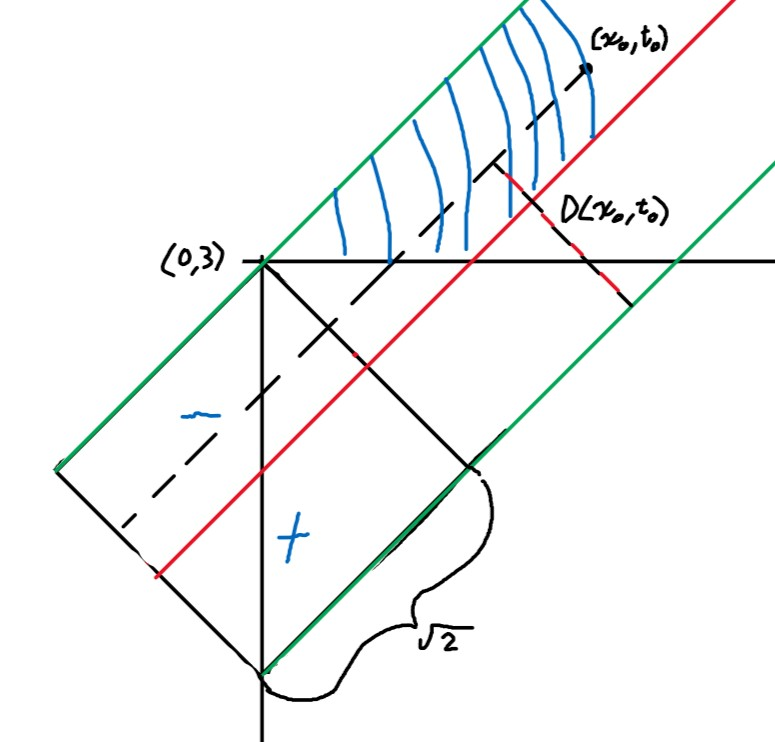
\includegraphics[scale=0.4]{30.jpg}
      %     \caption{On the right side of the red line, the domain of dependence does not intersect with the support of $f$ (black square) so $u(x,t) = 0$ , but on the left side of the red line, the domain of dependence of $u(x,t)$ contains the entire support of $f$ so the integral will be zero as it is $-1$ on the left side and $1$ on the right side (denoted by the + and - signs in blue).}
      %     For $(x_0,t_0)$ in the blue region, it only depends on $D(x_0,t_0)$, the red/black segment because it determines how much of the support of $f$ lies in the domain of dependence of $u(x_0,t_0)$. If $D = 0$, then $u(x_0,t_0) = 0$ (it lies on the left green line). If $D = \sqrt{2}$, then $u(x_0,t_0) = 0$ (it lies on the right green line). Because $f$ is balanced, then 
      %     we have that 
      %     \[u(x_0,t_0) = \begin{cases}
      %       D\sqrt{2} &0\le D \le \frac{\sqrt{2}}{2} \\
      %       2-D\sqrt{2} &\frac{\sqrt{2}}{2} \le D \le \sqrt{2}.
      %     \end{cases}\]
      %     This means that $u$ looks like a triangular spike between $t = x+1$ and $t = x+3$.
      %   \end{figure}
      % \end{proof}
      % \exercise{31}{Evans 2.24}
      % \begin{proof}[Solution:]
      %   \begin{align*}
      %     k_t(t) &= \frac{\partial}{\partial t} \frac{1}{2} \int_{-\infty}^\infty u^2_t(x,t)dx = \int_{-\infty}^\infty u_t\cdot u_{tt}dx \\
      %     p_t(t) &= \frac{\partial}{\partial t} \frac{1}{2} \int_{-\infty}^\infty u^2_x(x,t)dx = \int_{-\infty}^\infty u_x\cdot u_{xt}dx =\int_{-\infty}^\infty \Delta u\cdot u_{t}dx 
      %   \end{align*}
      %   Then $k_t + p_t = \int_{-\infty}^\infty u_t\cdot(u_{tt} - u_{xx}) = 0$ so $k + p$ is constant.\newline
      %   Using D'Alembert's Formula, we have an explicit solution for $u$ so 
      %   \[k(t) - p(t) = \frac{1}{8}\int_{-\infty}^\infty(h(x+t) - h(x-t))^2 - (g'(x+t) + g'(x-t) + h(x+t) + h(x-t))^2dx \]
      %   Because $h$ and $g$ have compact support, let $A\subset \R$ with $A = \max\{\text{supp}(g),\text{supp}(h)\}$ so that the integral vanishes on $\R\setminus A$. This means that as $t\to\infty$, $k(t) - p(t)=0$ on $\R\setminus A$ so $k(t)=p(t)$ for all large enough times $t$.
      % \end{proof}
      % \exercise{32}{Show that there is at most one smooth solution of the given wave type equation.}
      % \begin{proof}[Solution:]
      %   Let $v,w$ be smooth solutions to the wave type equation. Now, let $u = v - w$. We see that $u$ solves the problem, 
      %   \[\begin{cases}
      %     u_{tt} - \nabla\cdot(A(x)\nabla u) = 0 &\text{in}\quad \R^n\times (0,\infty)\\
      %     u(x,0) = 0,\,\,u_t(x,0) = 0 &\text{in}\quad \R^n.
      %   \end{cases}\]
      %   Because $A(x) \le \Lambda$, we let $M \ge \Lambda$. Now, we create the backwards light cone with width larger than any speed of propagation this PDE may have in space, which is this bound of $A$, 
      %   \[C(x_0,t_0) = \{(x,t):|x-x_0| < M(t_0-t),t\in[0,t_0]\}.\]
      %   Now, to show uniqueness, we wish to show that over this light cone, the energy is decreasing.
      %   \begin{align*}
      %     E(t) &= \int_{B(C(x_0,t_0-t))} \frac{1}{2}u_t^2 + \frac{1}{2}\langle A(x)Du,Du\rangle dx \\
      %     \dot{E}(t) &= \int_{B(C(x_0,t_0-t))} u_tu_{tt} +\langle A(x)Du,Du_t\rangle dx - \frac{1}{2}\int_{\partial B(C(x_0,t_0-t))} (Mu_t^2 + \langle A(x)Du,Du\rangle) dS(x)
      %   \end{align*}
      %   For the $\dot{E}(t)$ term, we then use Green's Formula to get that 
      %   \begin{align*}
      %     \dot{E}(t) &= \int_{B(C(x_0,t_0-t))} u_tu_{tt} -u_t(\nabla\cdot(A(x)\nabla u)) dx \\
      %     &+\int_{\partial B(C(x_0,t_0-t))} \langle A(x)Du,\nu u_t\rangle dS(x) - \frac{1}{2}\int_{\partial B(C(x_0,t_0-t))} (Mu_t^2 + \langle A(x)Du,Du\rangle) dS(x)
      %   \end{align*}
      %   So to conclude uniqueness, we need to show that $|\langle A(x)Du,\nu\rangle u_t| \le \frac{1}{2}(Mu_t^2 + \langle A(x)Du,Du\rangle)$.
      %   \begin{align*}
      %     |\langle A(x)Du,\nu  u_t\rangle|\le^\star \frac{1}{2}\langle A(x)Du,Du\rangle + \frac{1}{2}\langle A(x)\nu u_t,\nu u_t\rangle \le \frac{1}{2}\langle A(x)Du,Du\rangle + \frac{M}{2}|u_t|^2
      %   \end{align*}
      %   From this we see that the energy is decreasing, so $u$ must be constant within the light cone $C$ as $e(t) \le e(0) = 0$.\newline
      %   Proof of $\star$: Let $\langle A(x)v, w\rangle = \langle v,w\rangle_A$,
      %   \begin{align*}
      %     &\langle v-w,v-w\rangle_A = \langle v,v\rangle_A - 2\langle v, w\rangle_A + \langle w,w\rangle_A \ge 0 \\
      %     &\langle v,v\rangle_A  + \langle w,w\rangle_A \ge 2\langle v, w\rangle_A \\
      %     &\langle A(x)v,v\rangle  + \langle A(x)w,w\rangle \ge 2\langle A(x)v, w\rangle
      %   \end{align*}
      % \end{proof}
      % \exercise{33}{Consider the initial value problem for the wave equation.}
      % \begin{proof}[Solution:]
      %   \begin{enumerate}
      %     \item Since $\phi,D\phi,\psi$ are all supported on $B(0,1)$,  $\phi,D\phi,\psi = 0$ outside of $\partial B(x,t)\cap B(0,1)$.
      %     By Kirchoff's formula,
      %     \[u(x,t) = \frac{1}{4\pi t^2} \int_{\partial B(x,t)\cap B(0,1)} \phi(y) + \nabla \phi(y)\cdot(y-x) + t\psi(y)dS(y)\]
      %     Because $\phi,D\phi,\psi$ are smooth and supported, they are bounded so we have that 
      %     \[|u(x,t)| \le \frac{1}{4\pi t^2} \int_{\partial B(x,t)\cap B(0,1)} \sup_x|\phi(y)| + \sup_x|\nabla \phi(y)|(x-y) + t\sup_x|\psi(y)|dS(y)\]
      %     which simplifies to, allowing $y-x = t$,
      %     \[ |u(x,t)| \le \frac{\sup_x|\phi(y)| + t\sup_x|\nabla \phi(y)|+t\sup_x|\psi(y)|}{4\pi t^2}\int_{\partial B(x,t)\cap B(0,1)}dS(y)\]
      %     Over the surface, we have that $\int_{\partial B(x,t)\cap B(0,1)}dS(y) = 4\pi(1)^2 = 4\pi$ so we get that 
      %     \[|u(x,t)|\le \frac{(\sup_x|\phi(y)| + t\sup_x|\nabla \phi(y)|+t\sup_x|\psi(y)|)}{t^2}\]
      %     $\partial B(x,t)\cap B(0,1) \subset B(x,t+1)\setminus\overline{B}(x,t-1)$ so $u(x,t) = 0$ outside of $B(0,t+1)\setminus\overline{B}(0,t-1)$ as the domain of dependence $B(0,1)$ travels with $x$.
      %     \item Let $u$ be a solution to the wave equation in $(0,T)$, then we see that 
      %     \[v_{tt} = u_{tt} + u_{tt},\,\,\Delta v = \Delta u + \Delta u \implies v_{tt} - \Delta v = 0\]
      %     then for the initial conditions, 
      %     \[v(x,0) = u(x,T) + u(x,T) = 2u(x,T),\,\, v_{t}(x,0) = u_{t}(x,T) - u_{t}(x,T) = 0.\]
      %     Hence $v$ also solves the wave equation.
      %     \item Let $f(x)$ be a bump function supported on $B(0,1)$, then let $\phi(x) = Mf(x)$. We also let $\psi(x) = 0$. Now we have that $\phi,\psi$ are compactly supported smooth functions on $B(0,1)$ so by part (a), $\sup_x|u(x,t)| \le C\frac{M + ctM}{t^2}$. Because this tends towards 0, for $\epsilon > 0$, there exists a $T$ such that $\sup_{x}|u(x,T)| \le \frac{\epsilon}{2}$.\newline 
      %     This function $u(x,T)$ becomes our initial data to the equation $v(x,t) = u(x,t+T) + u(x,t-T)$ such that $2u(x,T)$ is compactly supported on the annulus $B(0,T+1)\setminus \overline{B}(0,T-1)$ and $\|2u(x,T)\|,\|2\partial_xu(x,T)\| \le \epsilon$. This additionally guarantees that $v_t(x,0) = 0$ by part (b).\newline
      %     Now, as $t\to T$, we see that $\sup_x|v(x,T)| = \sup_x|u(x,2T) + u(x,0)| = \sup_x|u(x,2T) + \phi(x)| \ge M$.
      %   \end{enumerate}
      % \end{proof}
      % \exercise{34}{Solve using characteristics
      % \begin{enumerate}
      %   \item $x_1u_{x_1} + x_2u_{x_2} = 2u, \quad u(x_1,1) = g(x_1)$ 
      %   \item $x_1u_{x_1} + 2x_2u_{x_2} + u_{x_3} = 3u,\quad u(x_1,x_2,0) = g(x_1,x_2)$
      %   \item $uu_{x_1} + u_{x_2} = 1,\quad u(x_1,x_1) = \frac{1}{2}x_1$
      % \end{enumerate}}
      % \begin{proof}[Solution:]
      %   The $\mathbf{p}$ terms in these are not necessary as there is no gradient nonlinear term so
      %   \begin{enumerate}
      %     \item $x_1u_{x_1} + x_2u_{x_2} = 2u, \quad u(x_1,1) = g(x_1)$
      %     \item[] We see that $\mathbf{b} = (x_1,x_2)$ and $c = -2$. We have 
      %     \begin{align*}
      %       \begin{cases}
      %         \dot{x} = x \\
      %         \dot{z} = 2z
      %       \end{cases}
      %     \end{align*} 
      %     so 
      %     \begin{align*}
      %       \begin{cases}
      %         x = Ae^s\\
      %         z = Be^{2s}
      %       \end{cases}
      %     \end{align*}
      %     where $A$ is selected to be $(C, 1)$. Now, we see that $B = z(0) = u(x(0)) = u(C,1) = g(C)$. In order to recover $(x_1,x_2)$, select $s = \log{(x_2)}$ and $C = \frac{x_1}{x_2}$ so we see $(Ce^{\log{x_2}},e^{\log{x_2}}) = (x_1,x_2)$ and
      %     \[u(x_1,x_2) = z(\log(x_1)) = g\left(\frac{x_1}{x_2}\right)e^{2\log{x_2}} = g\left(\frac{x_1}{x_2}\right) x_2^2\]
      %     \item $x_1u_{x_1} + 2x_2u_{x_2} + u_{x_3} = 3u,\quad u(x_1,x_2,0) = g(x_1,x_2)$
      %     \item[] We see that $\mathbf{b} = (x_1,2x_2, 1)$ and $c = -3$. We have 
      %     \begin{align*}
      %       \begin{cases}
      %         \dot{x} = (x_1,2x_2,1) \\
      %         \dot{z} = 3z
      %       \end{cases}
      %     \end{align*} 
      %     so 
      %     \begin{align*}
      %       \begin{cases}
      %         x = (Ae^{s}, Be^{2s}, s)\\
      %         z = Ce^{3s}
      %       \end{cases}
      %     \end{align*}
      %     Now, we see that $C = z(0) = u(x(0)) = u(A,B, 0) = g(A,B)$. In order to recover $(x_1,x_2,x_3)$, select $s = x_3$ and $A = x_1e^{-x_3}$, $B = x_2e^{-x_3}$ so we see $x(s) = (x_1e^{-x_3}e^{x_3},x_2e^{-x_3}e^{x_3},x_3) = (x_1,x_2,x_3)$ and 
      %     \[u(x_1,x_2,x_3) = z(x_3) = g(x_1e^{-x_3},x_2e^{-x_3})e^{3x_3}\]
      %     \item $uu_{x_1} + u_{x_2} = 1,\quad u(x_1,x_1) = \frac{1}{2}x_1$
      %     \item[] We have that $F(p,z,x) = p\cdot(z,1) - 1$ where $p=(u_{x_1},u_{x_2})$ and $z=u$. This has derivatives
      %     \begin{align*}
      %       D_pF &= (z,1) \\
      %       D_xF &= 0 \\
      %       D_zF &= p_1
      %     \end{align*} 
      %     hence the characteristics are
      %     \begin{align*}
      %       \begin{cases}
      %         \dot{x} = (z,1) \\
      %         \dot{z} = 1
      %       \end{cases}
      %     \end{align*}
      %     let $z(s) = s + A$ and $x_2 = s$. Because $\dot{x}_1 = z = s+A$, let $x_1(s) = \frac{1}{2}(s+A)^2 + B$. Assume there is an $s$ such that $x_1(s)=x_2(s)=s$ so 
      %     \[s+A = z(s) = u(x(s)) = u(s,s) = \frac{1}{2}s\]
      %     by the prescribed conditions so $s = -2A$. 
      %     \[-2A = x_2(-2A) = x_1(-2A) = \frac{1}{2}A^2 + B\]
      %     so $B = -2A - \frac{1}{2}A^2$. This means we have that 
      %     \[x(s) = \left(\frac{1}{2}(s+A)^2 - 2A - \frac{1}{2}A^2, s\right) = \left(\frac{1}{2}s^2 + As - 2A, s\right)\]
      %     and $u\left(\frac{1}{2}s^2 + sc - 2c,s\right) = u(x(s)) = z(s) = s + A$. Finding $s,A$ such that $x(s)=(x_1,x_2)$ gives that 
      %     \[(x_1,x_2) = \left(\frac{1}{2}s^2+As-2A,s\right)\]
      %     so $x_2 = s$ and $x_1 = A(s-2) + \frac{1}{2}s^2$ which implies that $A = \frac{2x_1-x_2^2}{2(x_2-2)}$ which gives that 
      %     \[u(x_1,x_2) = x_2 + \frac{2x_1-x_2^2}{2(x_2-2)}.\]
      %   \end{enumerate}
      % \end{proof}
      % \exercise{35}{Consider the transport equation 
      % \[u_t + a(x,t)\cdot\nabla u = 0.\]
      % Show that if $u$ is a $C^1$ solution and $\beta : \R\to \R$ is an arbitrary $C^1$ function, then $\beta(u)$ is a solution as well.}
      % \begin{proof}[Solution:]
      %   \[\frac{d}{dt}\beta(u(x,t)) = \beta'(u(x,t)) u_t(x,t)\] and \[\nabla_x \beta(u(x,t)) = \beta'(u(x,t)) \nabla u(x,t)\] as $\frac{d}{dx_n} \beta(u(x,t)) = \beta'(u(x,t))u_{x_n}(x,t)$ for each $n$. Now, 
      %   \[\frac{d}{dt}\beta(u(x,t)) + a(x,t)\cdot \nabla_x \beta(u(x,t)) = \beta'(u(x,t))\left(u_t(x,t)+ a(x,t)\cdot \nabla u(x,t)\right) = \beta'(u(x,t))\cdot 0 = 0.\]
      % \end{proof}
      % \exercise{36}{Find the characteristics for the problem 
      % \[u_t - \frac{1}{2}u_x^2 - \frac{1}{2}x^2 = 0\] with initial condition $u(x,0) = x$. Explain why the solution is not defined for $|t|\ge \pi/2$.}
      % \begin{proof}[Solution:]
      %   % Finding the derivative in $x$ we see $u_{tx} - u_xu_{xx} - x = 0$. Let $v = u_x$ so we see that 
      %   % \[v_t - vv_x -x = 0\] with $v(x,0) = 1$. Letting $q = v_x$, $p=v_t$, $z=v$, we have that 
      %   % \[F(p,q,z,x) = p - zq - x = 0\]
      %   % with characteristics 
      %   % \begin{align*}
      %   %   \begin{cases}
      %   %     \dot{z} = q\partial_q F + p\partial_p F = p - zq = x \\
      %   %     \dot{x} = \partial_q F = -z.
      %   %   \end{cases}
      %   % \end{align*}
      %   % with initial data $x(t=0) = A$, $z(A,0) = 1$. Moreover, we see that 
      %   % \[\ddot{x} = \frac{d}{dt}\dot{x} = -\dot{z} = -x\]
      %   % so letting $(x(0), z(0)) = (A, 1)$, 
      %   % \[x(t) = \sin(t) + A\cos(t)\]
      %   %  which means 
      %   %  \[z(t) = \cos(t) - A\sin(t)\]
      %   Abusing notation with $(t,x) = (x_1,x_2)$, rewrite this as $F(p,z,x) = p_1 - \frac{1}{2}p_2^2 - \frac{1}{2}x_2^2$.
      %   \begin{align*}
      %     \dot{p}_1(s) &= 0, \,\,\dot{p}_2(s) = x_2 \\
      %     \dot{z}(s) &= (1, -p_2)\cdot(p_1,p_2) = p_1 - p_2^2 \\
      %     \dot{x}_1(s) &= 1, \,\,\dot{x}_2(s) = -p_2
      %   \end{align*}
      %   Then we have that $p_1(s) = p_1^0$, $x_1(s) = x_1^0 + s=s$ and the following system
      %   \begin{align*}
      %     \begin{bmatrix}
      %       \dot{x_2} \\
      %       \dot{p_2}
      %     \end{bmatrix} = 
      %     \begin{bmatrix}
      %       0 & -1 \\
      %       1 & 0
      %     \end{bmatrix}\begin{bmatrix}
      %       {x_2} \\
      %       {p_2}
      %     \end{bmatrix}
      %   \end{align*}
      %   which has solutions $(x_2(s),p_2(s)) = (A\cos(s)-B\sin(s),-A\sin(s)-B\cos(s))$.
      %   To find $A,B$, $p_2^0 = u_x(x_0,0) = \frac{d}{dx} x = 1$ and $x_2^0 = x_0$ where $x_0\in \R$. This means we have the following characteristic 
      %   \[x(s) = x_0\cos(s) - \sin(s).\]
      %   Perturbing $x_0$ we see in the following figure that they cross at some value $t$ (where $t$ is the y-axis and $x$ is the x-axis)
      %   \begin{figure}[H]
      %     \centering
      %     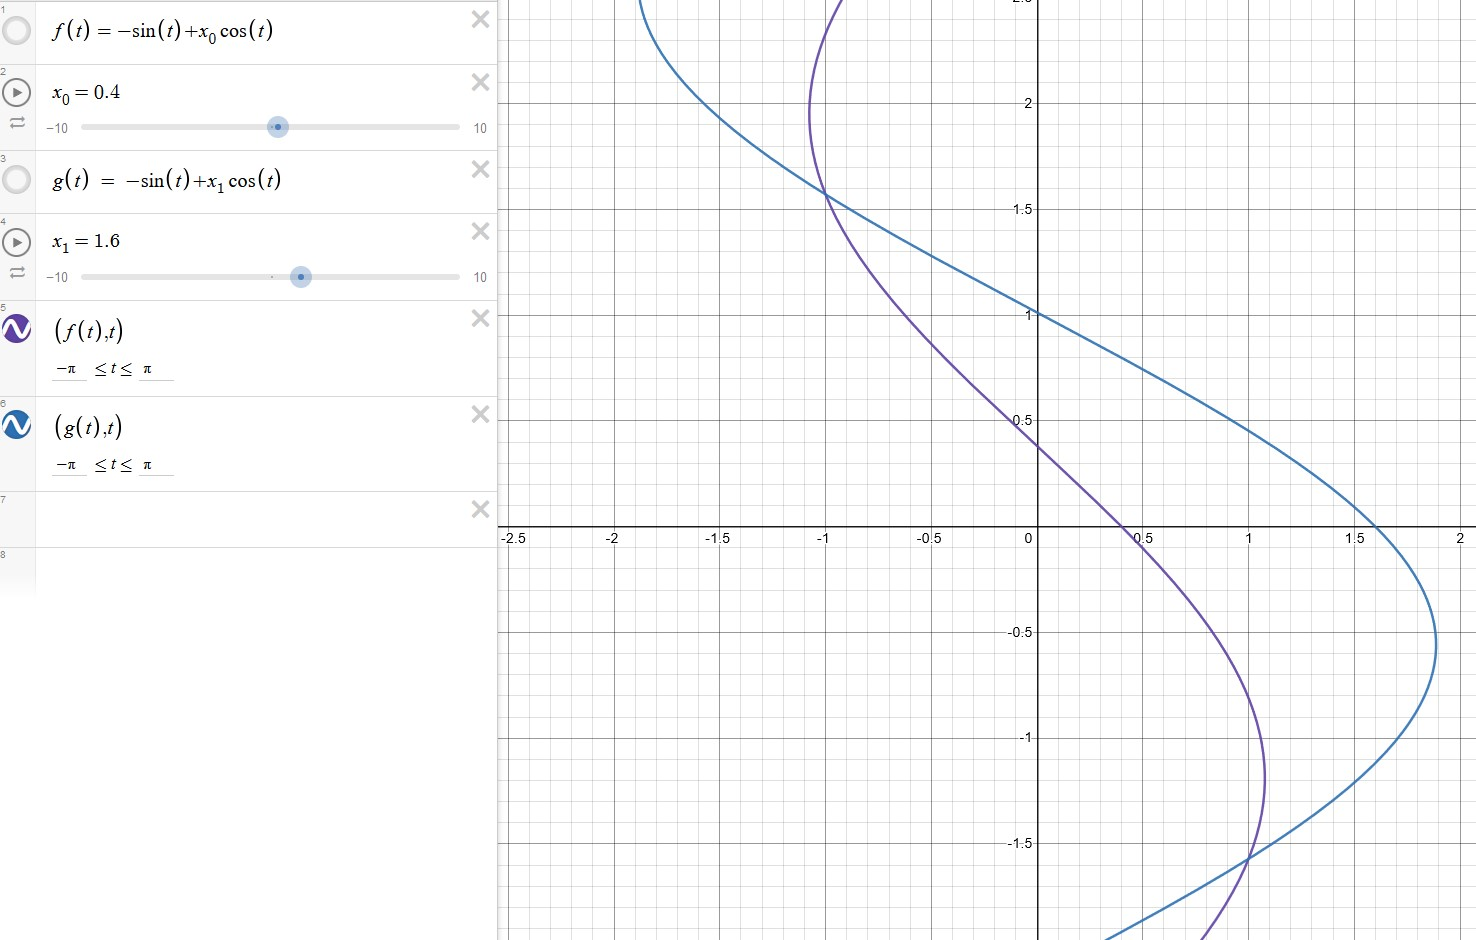
\includegraphics[scale=0.3]{36.jpg}
      %   \end{figure}
      % \end{proof}
      % \begin{align*}
      %   x_1 \cos(s) - \sin(s) = x_0\cos(s) - \sin(s) \\
      %   \cos(s)(x_1-x_0) = 0
      % \end{align*}
      % which implies $|s| = \pi/2$ for the first time where they intersect. This means that there is no existence for $|t| \ge \pi/2$.
    % \exercise{37}{Consider the solution of Burger's equation with smooth initial data $u_0$
    % \begin{enumerate}
    %   \item Compute, in terms of $u_0$, the first time $t_\star$ when characteristics cross.
    %   \item Derive a necessary and sufficient condition on $u_0$ so that $t_\star = +\infty$.
    % \end{enumerate}}
    % \begin{proof}[Solution:]
    %   Using $q=u_t$, $p=u_x$, and $z=u$ so we have 
    %   \[q + zp = 0\]
    %   This has characteristic ODEs 
    %   \begin{align*}
    %     \dot{x} = z \\
    %     \dot{z} = 0
    %   \end{align*}
    %   This has solution 
    %   \begin{align*}
    %     x(t) = zt + A \\
    %     z(t) = B
    %   \end{align*}
    %   where $B$ is a function of $A$. The characteristics of $x$ have that following 
    %   \[x(t) = u(x(0),0)t + x(0) = u_0(x_0)t + x_0.\]
    %   For general initial $x_1,x_0\in\R$ we have an intersection when 
    %   \begin{align*}
    %     u_0(x_1)t_\star + x_1 &= u_0(x_0)t_\star + x_0 \\
    %     t_\star &= \frac{x_1-x_0}{u_0(x_1)-u_0(x_0)}.
    %   \end{align*}
    %   We see that $t_\star \to\infty$ whenever $u_0(x_1) - u_0(x_0)$ is sufficiently small, but because $x_1$ and $x_0$ are arbitrary, $u_0$ must be constant.
    % \end{proof}
    % \exercise{38}{Consider the scalar conservation law with initial data $u(x,0) = -x$. Show that if $f''(z) \ge \theta > 0$ for all $z\in \R$ then $\inf_{x\in\R} \partial_xu(x,t)\to-\infty$ in a finite time.}
    % \begin{proof}[Solution:]
    %   The conservation law can be written as 
    %   \[u_t + F'(u)u_x = 0\]
    %   so it has characteristic
    %   \begin{align*}
    %     \begin{cases}
    %       \dot{p}(t) = - F''(z(t))p(t)^2
    %     \end{cases}
    %   \end{align*}
    %   where $z = u$ and $p = u_x$. Now, because $F''(z) \ge \theta > 0$, we have the differential inequality
    %   \[\dot{p}(t) \le - \theta p(t)^2\]
    %   which means that  
    %   \[ -\frac{1}{p(t)} \le C-\theta t \implies p(t) \le -\frac{1}{C-\theta t}\]
    % $p(0) = -1$ ($(-x)_x$) so we see that $C=1$ so 
    % \[p(t) \le -\frac{1}{1-\theta t}.\]
    % $p(t)$ then tends towards $-\infty$ in $t^\star = \frac{1}{\theta}$.
    % \end{proof}
    % \exercise{39}{Evans Chapter 3 problem 19}
    % \begin{proof}[Solution:]
    %   Because $u$ is a continuous integral solution, we can look at solutions to the problem when time starts at $s$
    %   \begin{align*}
    %     \begin{cases}
    %       u_t + F(u)_x = 0 &\text{ in $\R\times (\tau,\infty)$} \\
    %       u = u(x,\tau) &\text{on $\R$},
    %     \end{cases}
    %   \end{align*} 
    %   and these still have an integral solution 
    %   \[\int_\tau^\infty \int_{\R}(uv_t + F(u)v_x)dxdt + \int_{\R}uvdx\vert_{t=\tau} = 0,\]
    %   for $v\in C^\infty_c(\R\times[\tau,\infty))$. The difference between this and the original integral solution is 
    %   \[\int_0^\tau\int_{\R}uv_t + F(u)v_xdxdt + \int_\R gvdx\vert_{t=0} - \int_{\R} uvdx\vert_{t=\tau} = 0.\]
    %   Because $F(0)=0$, we notice $F(u(x\to\infty, t)) = F(0) = 0$ so $F$ is compactly supported as $u$ is compactly supported. Let $v = 1$ over the support of $u$ union the support of $F$. This eliminates the double integral term so we're left with 
    %   \[\int_\R gvdx\vert_{t=0} = \int_\R uvdx\vert_{t=\tau} \implies \int_\R gdx = \int_\R u(x,\tau)dx\]
    %   from our choice of $v = 1$.
    % \end{proof}
    % \exercise{40}{Entropy Solutions of Scalar Conservation Law}
    \exercise{41}{Evans Chapter 3 Problem 20}
    \begin{proof}[Solution:]
      There is a shock at $x=-1$ and $x=1$, and there is a rarefaction at $x=0$. From the Rankine-Hugoniot condition, at $x=-1$, $\sigma = \frac{1}{2}$ and at $x=1$, $\sigma = 1$.
      This would then have solution 
      \[u(x,t) = \begin{cases}
        1 &x<-1+\frac{1}{2}t \\
        0 &-1+\frac{1}{2}t < x < 0 \\
        \frac{x}{t} &0 < x < 2t \\
        2 &2t < x < 1+t \\
        0 &x > 1+t
      \end{cases}\]
      However, we see that there are collisions at $t=2$ and $t=1$, so solutions for this only exists for $0\le t \le 1$. For the shock at $t=1$, we have that $u_l = \frac{x}{t}$ and $u_r = 0$ so then 
      \[\dot{s}(t) = \frac{\frac{1}{2}\left(\frac{s(t)}{t}\right)^2}{\frac{s(t)}{t}} = \frac{s(t)}{2t} \implies s(t) = 2\sqrt{t}\]
      as $s(1) = 2$. Then when $t = 2$, we have that $u_l = 1$ and $u_r = \frac{x}{t}$ so 
      \[\dot{q}(t) = \frac{1}{2}\frac{1 - \left(\frac{q(t)}{t}\right)^2}{1-\frac{q(t)}{t}} = \frac{1}{2}(1+\frac{q(t)}{t})\implies q(t) = t - \sqrt{2t}\]
      as $q(2) = 0$. $q(t) = s(t)$ when $t = 6 +4\sqrt{2}$ so there will be another shock there. Moreover, for $1 \le t \le 2$, we have that solution 
      \[u(x,t) = \begin{cases}
        1 &x<-1+\frac{1}{2}t \\
        0 &-1+\frac{1}{2}t < x < 0 \\
        \frac{x}{t} &0 < x < 2\sqrt{t} \\
        0 &x > 2\sqrt{t}
      \end{cases}\]
      and for $2\ge t \ge 6+4\sqrt{2}$
      \[u(x,t) = \begin{cases}
        1 &x<t - \sqrt{2t}\\
        \frac{x}{t} &t - \sqrt{2t} < x < 2\sqrt{t} \\
        0 &x > 2\sqrt{t}
      \end{cases}\]
      Finally, the shock at $t = 6+4\sqrt{2}$ is given by $u_l = 1$ and $u_r=0$ with 
      \[\dot{r}(t) = \frac{1}{2} \implies r(t) = \frac{1}{2}t + 1\]
      as $r(6+4\sqrt{2}) = 4+2\sqrt{2}$. The solution for $t > 6+4\sqrt{2}$ is given by 
      \[u(x,t) = \begin{cases}
        1 &x<1 + \frac{1}{2}t\\
        0 &x > 1 + \frac{1}{2}t.
      \end{cases}\]
      The shocks are given by 
      \begin{figure}[H]
        \centering
        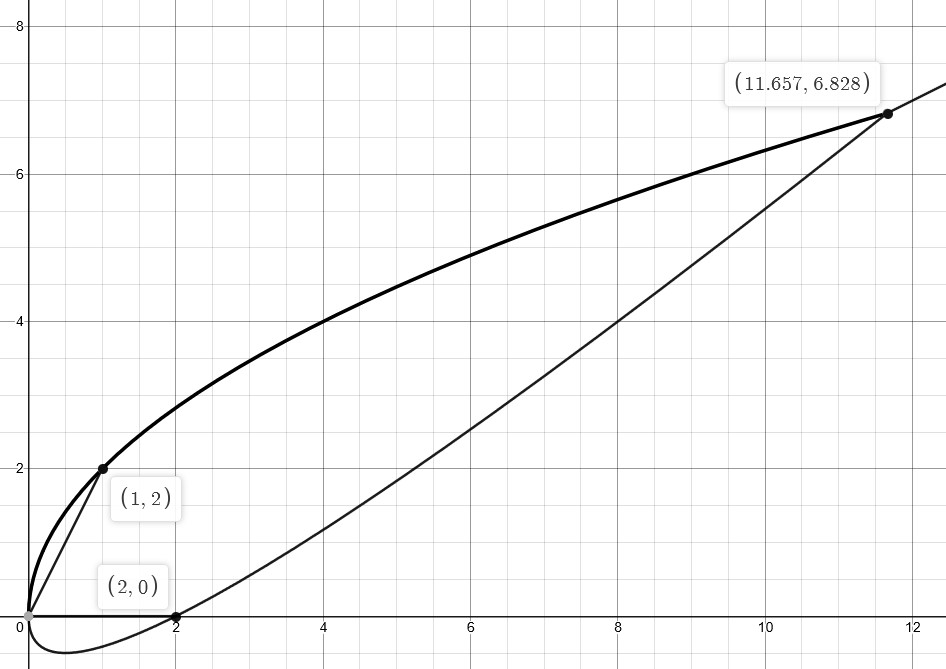
\includegraphics[scale=0.5]{shocks.jpg}
        \caption{Plotted are the shocks. Time is on the $x-axis$ and $x$ is on the $y-axis$. There are collisions at $t=1,2$ and $t=6+4\sqrt{2}$.}
      \end{figure}
    \end{proof}
    \exercise{42}{Evans Chapter 3 Problem 9}
    \begin{proof}[Solution:]
      \begin{enumerate}[(a)]
        \item Define $\mathcal{S} = \{y\in C^\infty|y(0)=y(t)=0\}$ and $i : \R\to\R$ such that 
        \[i(\epsilon) = \int_0^t L(\dot{x}(s) + \epsilon \dot{y}(s), x(s)+\epsilon y(s))ds.\]
        Now, $i$ has a inimum at $\epsilon = 0$ so 
        \[i'(0) = \int_0^t\sum_{j=1}^n L_{v_j}(\dot{x},x)\dot{y}_j + L_{x_j}(\dot{x},x)y_jds = 0.\]
        Then, by integration by parts, 
        \begin{align*}
          L_{v_j}(\dot{x}(t),x(t))y_j - L_{v_j}(\dot{x}(0),x(0))y_j(0) &= \int_0^t \left[\frac{\partial}{\partial s}L_{v_j}(\dot{x},x)y_j\right]ds \\
          &= \int_0^t \left[\left(\frac{\partial}{\partial s}L_{v_j}(\dot{x},x)\right)y_j + L_{v_j}(\dot{x},x)\dot{y}_j\right]ds = 0.
        \end{align*}
        This gives that 
        \[\int_0^t L_{v_j}(\dot{x},x)\dot{y}_j = - \int_0^t\left(\frac{\partial}{\partial s} L_{v_j}(\dot{x},x)\right)y_jds\]
        Putting this into $i'(0)$, we see that 
        \[\sum_{j=1}^n\int_0^t \left[-\frac{\partial}{\partial s} L_{v_j}(\dot{x},x) + L_{x_j}(\dot{x},x)\right]y_jds = 0\]
        which implies that for all $j=1,2,\dots,n$,
        \[-\frac{\partial}{\partial s}L_{v_j}(\dot{x},x) + L_{x_j}(\dot{x},x) = 0\]
        as $y\in \mathcal{S}$ was arbitrary. Hence,  $x(s)$ satisfies the Euler-Lagrange Equations.
        \item Now let $\mathcal{S} = \{y\in C^\infty, y(t)=0\}$. For any $y\in \mathcal{S}$ and $\epsilon\in\R$, $x+\epsilon y \in \mathcal{A}$, so $i(\epsilon)$ has a minimum at $\epsilon = 0$ for any fixed $y\in \mathcal{S}$. By integration by parts, 
        \[-L_{v_j}(\dot{x}(0),x(0))y_j(0) = \int_0^t\left[\left(\frac{\partial}{\partial s} L_{v_j}(\dot{x},x)\right)y_j+L_{v_j}(\dot{x},x)\dot{y}_j\right]ds \]
        Therefore, 
        \[ \int_0^t L_{v_j}(\dot{x},x)\dot{y}_jds = -L_{v_j}(\dot{x}(0),x(0))y_j(0)-\int_0^t\left[\left(\frac{\partial}{\partial s} L_{v_j}(\dot{x},x)\right)y_j(s)\right]ds\]
        If we put this equality into $i'(0)$ we have that 
        \[\sum_{j=1}^n\int_0^t \left[-\frac{\partial}{\partial s}L_{v_j}(\dot{x},x) + L_{x_j}(\dot{x},x)\right]y_jds - D_vL(\dot{x}(0),x(0))\cdot y(0) = 0\]
        Using part (a), we see that $D_vL(\dot{x}(0),x(0))\cdot y(0) = 0$ for any $y\in \mathcal{S}$, thus $D_vL(\dot{x}(0),x(0)) = 0$.
        \item For any $y \in \{y\in C^\infty|y(0)=y(t)=0\}$ and $\epsilon \in \R$, $x + \epsilon y \in \mathcal{A}$ and $g(x(0)) = g(x(0) + \epsilon y(0))$. Define $k:\R\to\R$ such that 
        \[k(\epsilon) = i(\epsilon) + g(x(0) + \epsilon y(0)) = \int_0^t L(\dot{x} + \epsilon\dot{y},x + \epsilon y)ds + g(x(0) + \epsilon y(0)).\]
        By similar reasoning from (a), 
        \[ k'(0) = \sum_{j=1}^n \int_0^t \left[-\frac{\partial}{\partial s}L_{v_j}(\dot{x},x) + L_{x_j}(\dot{x},x)\right]y_jds\]
        because $g(x(0)+\epsilon y(0))$ is constant as $\epsilon$ changes. Therefore $x$ satisfies the Euler-Lagrange Equations. Now consider $y\in \{y\in C^\infty, y(t)=0\}$, and define $k(\epsilon)$ in the same way. Then we see that 
        \[k'(\epsilon) = i'(\epsilon) + \frac{\partial}{\partial \epsilon}g(x(0) + \epsilon y(0)) = i'(\epsilon) + Dg(x(0) + \epsilon y(0))\cdot y(0)\]
        so at $\epsilon = 0$, $k'(0) = i'(0) + Dg(x(0))\cdot y(0)$. From $b$ we know that $i'(0) = -D_vL(\dot{x}(0), x(0))\cdot y(0)$ since $x$ satisfies the E-L equations. Therefore, 
        \[k'(0) = -D_vL(\dot{x}(0),x(0))\cdot y(0) + Dg(x(0)) \cdot y(0) = (Dg(x(0)) - D_vL(\dot{x}(0),x(0)))\cdot y(0) = 0.\]
        Because this holds for all $y$, we have that $D_vL(\dot{x}(0),x(0)) = Dg(x(0))$ as an initial condition for minimizers $x$.
      \end{enumerate}
    \end{proof}
    \exercise{43}{Evans Chapter 3 Problem 10}
    \begin{proof}[Solution:]
      We have that $L(v) = \sup_{p\in \R^n}[v\cdot p - H(p)] = \sup_{p\in\R^n} \left[v\cdot p - \frac{|p|^r}{r}\right].$
      We can then use Young's inequality with $\frac{1}{r}+\frac{1}{s}=1$,
      \[v\cdot p \le |v||p| \le \frac{|p|^r}{r} + \frac{|v|^s}{s}\]
      so 
      \[L(v) = \sup_{p\in\R^n}\left[v\cdot p - \frac{|p|^r}{r}\right] \le \frac{|v|^s}{s}.\]
      Let $p = v|v|^{(s-r)/r}$ so 
      \begin{align*}
        v\cdot p - \frac{|p|^r}{r} &= v\cdot v|v|^{(s-r)/r} - \frac{|v|v|^{(s-r)/r}|^r}{r} \\
        &= |v|^{(s+r)/r} - \frac{|v|^s}{r} \\
        &= |v|^s - \frac{|v|^s}{r} = \frac{|v|^s}{s}.
      \end{align*}
      using that $\frac{1}{s} + \frac{1}{r} = 1$. This implies that $L(v) = \frac{|v|^s}{s}$.\newline
      Now, fix $v\in \R^n$ and define $f = f_v : \R^n \to \R$ with 
      \[f(p) = v\cdot p - H(p) = \sum_{i=1}^n(v_i - b_i)p_i - \frac{1}{2}\sum_{i,j=1}^n a_{ij}p_ip_j\]
      If $f$ is bounded, then there is a $p^\star$ such that $f(p^\star) = \sup_{p\in\R^n} f(p) = L(v)$. Because $f$ is smooth, $p^\star$ must be a critical point with $Df(p^\star) = 0$. Let $r_i$ be the $i$th row of the matrix $A$, then 
      \[\frac{\partial}{\partial p_i} f(p^\star) = (v_i - b_i) - r_i\cdot p^\star\]
      Hence, 
      \[Df(p^\star) = v - b - Ap^\star.\]
      Because $A$ is positive definite, it is invertible, so $p^\star = A^{-1}(v-b)$. Moreover, the Hession of $f$ at $p^\star$ is $-A$, which is negative definite so $p$ is a global maximum (as it was assumed that it was the only critical point of $f$). Therefore, 
      \begin{align*}
        L(v) &= f(p^\star) \\
        &= (v-b)\cdot p^\star - \frac{1}{2}(p^\star)^T A p^\star \\
        &= (v-b)\cdot(A^{-1}(v-b)) - \frac{1}{2}(A^{-1}(v-b))^T A (A^{-1}(v-b)) \\
        &= (v-b)\cdot(A^{-1}(v-b)) - \frac{1}{2}((v-b)^TA^{-1}) A (A^{-1}(v-b)) \\
        &= \frac{1}{2}(v-b)^TA^{-1}(v-b).
      \end{align*}
      Now all is left is to show that $f$ is bounded.\newline
      $x^T A x$ is continuous so we can choose some $x^T A x \ge M > 0$ for $|x| = 1$. Let $p_1 = \frac{p}{|p|}$ so 
      \begin{align*}
        f(p) &= (v-b)\cdot p - p^T A p \\
        &\le |v-b||p| - |p|^2 p_1^T A p_1 \\
        &\le|v-b||p| - M|p|^2\\
        &= \frac{1}{M}M|p|(|v-b| - M|p|)\\
        &\le \frac{1}{M}\frac{|v-b|^2}{4}.
      \end{align*}
    \end{proof}
    \exercise{44}{Evans Chapter 3 Problem 13}
    \begin{proof}[Solution:]
      Define $f(y) = tL(\frac{x-y}{t}) + g(y)$ and assume $f$ takes its minimum at some $y_0$. This means $Df(y_0) = 0$. We know that $Df(y) = -tDL(\frac{x-y}{t})\frac{1}{t} + Dg(y) = Dg(y) - DL(\frac{x-y}{t})$ so we have that 
      \[DL(\frac{x-y_0}{t}) = Dg(y_0).\] Then, by (16) in Theorem 3 in 3.3.2, $DH(Dg(y_0)) = DH(DL(\frac{x-y_0}{t}))=\frac{x - y_0}{t}$. We are given that $R \ge |DH(Dg)|$ so we have that 
      \[Rt \ge |x-y_0|\]
      so $y_0 \in B(x,Rt)$ meaning that 
      \[\min_{y\in\R^n} \left[tL(\frac{x-y}{t}) + g(y)\right] = \min_{y\in B(x,Rt)}\left[tL(\frac{x-y}{t}) + g(y)\right].\]

    \end{proof}
    \exercise{45}{Evans Chapter 3 Problem 14}
    \begin{proof}[Solution:]
      $L(v) = \min_{p\in\R^n} [v\cdot p - |p|^2] \le |v||p| - |p|^2 \le \frac{|v|^2}{4} + |p|^2 - |p|^2 = \frac{|v|^2}{4}.$ However, for $p^\star = \frac{v}{2}, p^\star \cdot v - |p^\star|^2 = \frac{|v|^2}{4}$. This means that 
      \[L(v) = \frac{|v|^2}{4}.\]
      Now, write $u$ as the Hopf-lax formula, 
      \begin{align*}
        u(x,t) &= \min_{y\in\R^n} \left[tL(\frac{x-y}{t}) + g(y))\right]\\
        &= \min_{y\in\R^n} \left[\frac{|x-y|^2}{4t} + g(y))\right]
      \end{align*}
      Using the given $g(y) = u(y,0)$, 
      \[ u(x,t) = \min_{y\in E} \left[\frac{|x-y|^2}{4t}\right] = \frac{1}{4t}\operatorname{dist}(x,E)^2.\]
    \end{proof}  
    \end{document}